\chapter{British linguistics and Firthian prosodic analysis}
\label{ch.firth}

Preceding chapters have been primarily concerned with the development
of pho\-nological theory in continental Europe; those that follow will
trace its evolution in North America. The present chapter is devoted
to a summary sketch of the approaches to \isi{sound structure} taken by
linguists in Great Britain during the same period; but its location in
the exposition should not in the least be taken as a claim that
British linguistics somehow forms a bridge or connection between these
other two major traditions. If anything, the very independence of the
theories to be discussed here from either the continental European or
the North American models will serve to emphasize the separateness of
these two main components of the present book.

The study of \isi{sound structure} in Britain (generally referred to there
as \emph{phonetics}, whether or not it also includes the material
called phonology by others) warrants a book-length study of its own,
by virtue both of its long history and of the theoretical novelties it
presents. For the modern linguist, the aspect of this history that is
most intriguing is the theory of \emph{Prosodic Analysis} associated
with J. R. {\Firth} and his students at the School of Oriental and
African Studies in London University; but the origins of this view and
its relation to the phonetic tradition represented by such great names
as \name{Henry}{Sweet} and \name{Daniel}{Jones} would surely be worth exploring as
well.  Prior to the 1970s, there were few general discussions of
\isi{prosodic analysis} and its background beyond the brief sketches of
\citet{robins:prosodic,robins:ling_in_gb} and the critical summary
(from the point of view of early generative phonology) by
\citet{langendoen68:london.school}.  More general recent accounts of
the history of linguistics in Britain up until the 1960s include that
of \citet{matthews99:philsoc}, the personal histories collected by
\citet{brown.law02:lx.in.uk} and a series of studies of Firthian
themes edited by \citet{kelly.plug05:firthian}.

If there are two features which characterize the study of language in
Britain up until the early 1960s, these are its insularity and an
emphasis on pragmatism rather than principles. Indeed, while linguists
elsewhere would probably resent having either of these attributes
associated with their work, British writers have often shown what
seems to others a strange pride in the completely homegrown character
of their tradition, and its emphasis on the practical and the \emph{ad hoc}
at the expense of broad conceptual and theoretical results.

The British certainly were not the first to concern themselves with
the nature and relations of the sounds of language, but as pointed out
in detail by \citet{firth46:english.school} and
\citet{abercrombie48:forgotten}, this study has a particularly long
and important past in the work of {English} grammarians, orthoepists,
and other scholars going back to the sixteenth century and
beyond. This tradition concerned itself largely with the study of
\ili{English}, and was to a great extent self-contained rather than
developing in relation to comparable scholarship elsewhere.

This concentration on the apparently local problem of the description
of \ili{English}, in the general context of British independence in
scientific and philosophical inquiry, was coupled in some cases with
personal attitudes: \name{Henry}{Sweet}, for example, had a highly unfavorable
opinion of the methods and results of {German} philological scholarship,
and set out specifically to provide a viable (and suitably British)
alternative to it. Over time, a model for the scientific investigation
of language arose which took its problems, its methods, and the
criteria for its critical evaluation almost exclusively from British
sources— resulting in a growing lack of connection with work being
done anywhere else.

As late as 1969, \citeauthor{robins69:rvw.langendoen} could suggest
(in a review of \citealt{langendoen68:london.school}) that the fact
that neither {\Firth} nor any of his students attempted an ``adequate
statement of his linguistic theories \ldots\ must in part be
attributed to the lack of an adequate challenge to Firthian
linguistics during the Firthian period.'' True, ``American linguists
were little interested in British development,'' and perhaps the
general level of international scholarly interchange was lower than
what we are accustomed to today—but it is at least equally clear that
British linguists showed little or no interest in seeking such
interchange. If there was no effective alternative to {\Firth} in British
linguistics, and thus no stimulus to him to clarify his position, this
was because the possibility of looking for such alternatives outside
Britain itself was not the kind of thing to be seriously pursued.

The pragmatic character of British approaches to scientific
linguistics was aptly summed up by \citet{householder52:rvw.jones} in
his review of Daniel \posscitet{jones50:phoneme} book \textsl{The
  Phoneme}: ``The European asks: `Is it true?', the American: `Is it
consistent?', the Englishman: `Will it help?'\,'' {\Jones}'s book, for
example, has a subtitle promising to describe, for the \isi{phoneme},
\textsl{Its Nature and Use}, and it quickly becomes clear that a
primary consideration for him in choosing among theoretical views of
the \isi{phoneme} is the question of which approach yields the most
immediate benefits in areas such as language teaching. Indeed, a
fundamental motivation for phonetic research in Britain, from the
early orthoepists through Bell\ia{Bell, Alexander Melville}, {\Sweet}, and {\Jones} was the issue of how
to teach the pronunciation of foreign languages. Benefits for our
theoretical understanding of the nature of language in general were
definitely of subsidiary (even though not inconsiderable) interest in
this enterprise.

A similar eschewal of abstract theoretical concerns for practical ones
can be identified in the commitment on the part of {\Firth} and his
students to `poly-systemic' analyses. As we will discuss below, the
content of this is the claim that whatever sort of analysis works best
in a given limited area should be adopted for that area—even if this
analysis is unrelated to or, worse, inconsistent with the analysis
provided for some other area of the same language. There is no reason
at all, on this view, to present a unified or coherent picture of an
entire language insofar as particular disconnected approaches to it
yield better results in limited areas.

As a consequence of this concern with results rather than general
principles, most of the concerns of both continental European and
North American scholarship about language have seemed foreign to
British linguists— even those who felt motivated to explore other
approaches—and vice versa. It is thus somewhat forced to present the
development of linguistics in Great Britain in the present context,
given the extent to which our attention has been dominated by
questions of little essential interest to the major figures in 
linguistics in Britain during the period under consideration.

Trends in the 1960s and 1970s, illustrated by the activities of
organizations such as the Linguistic Association of Great Britain and
its publications including the \textsl{Journal of Linguistics} have
largely reversed this tendency to
isolation.\footnote{\citet{matthews99:philsoc} also associates the
  shift in attention on the part of British linguists to more
  international themes with the rise of the LAGB and its partial
  replacement of the Philological Society. His account makes clear,
  however, that the theoretical work of figures such as {\Saussure},
  {\Trubetzkoy}, {\Hjelmslev}, {\Bloomfield} and others was by no means
  disregarded in the years prior to the 1960s.} By the end of the 20th
century, linguists in the United Kingdom were as well integrated into
the field in international terms as those of any other country.

Nonetheless, there are several areas in which earlier British research
provides essential perspective on the work of other schools. First,
\name{Daniel}{Jones}'s theory of the \isi{phoneme} provides us with a new conceptual
foundation for this element, one not covered by the classification
suggested in chapter~\ref{ch.saussure_sound} but which is quite close
to the view that would later become the consensus position for many
American structuralists. Secondly, British linguistics has
consistently been much more thoroughly based on detailed, accurate
phonetic observation than work elsewhere, and is important to an
understanding of the relation between phonetics and phonology.

Third, {\Firth}'s work was essentially the only major approach to
linguistics in the period 1935-57, which questioned the central role
of the \isi{phoneme} in phonological analysis. And in addition, the
introduction by {\Firth} and his students of the notion of `prosodies'
anticipates in many ways post-\textsl{SPE} developments in generative
phonology including aspects of Autosegmental and Metrical theory
(cf. chapter~\ref{ch.otlabphon}, though see
\citet{ogden.local94:misrepresentation} for some limitations of the
parallel. The similarities and differences between these pictures
certainly merit more than the minimal discussion which considerations
of space allow us below.

\section{Henry Sweet, Daniel Jones, and the British phonetic tradition}

\begin{wrapfigure}{r}{.4\textwidth}
  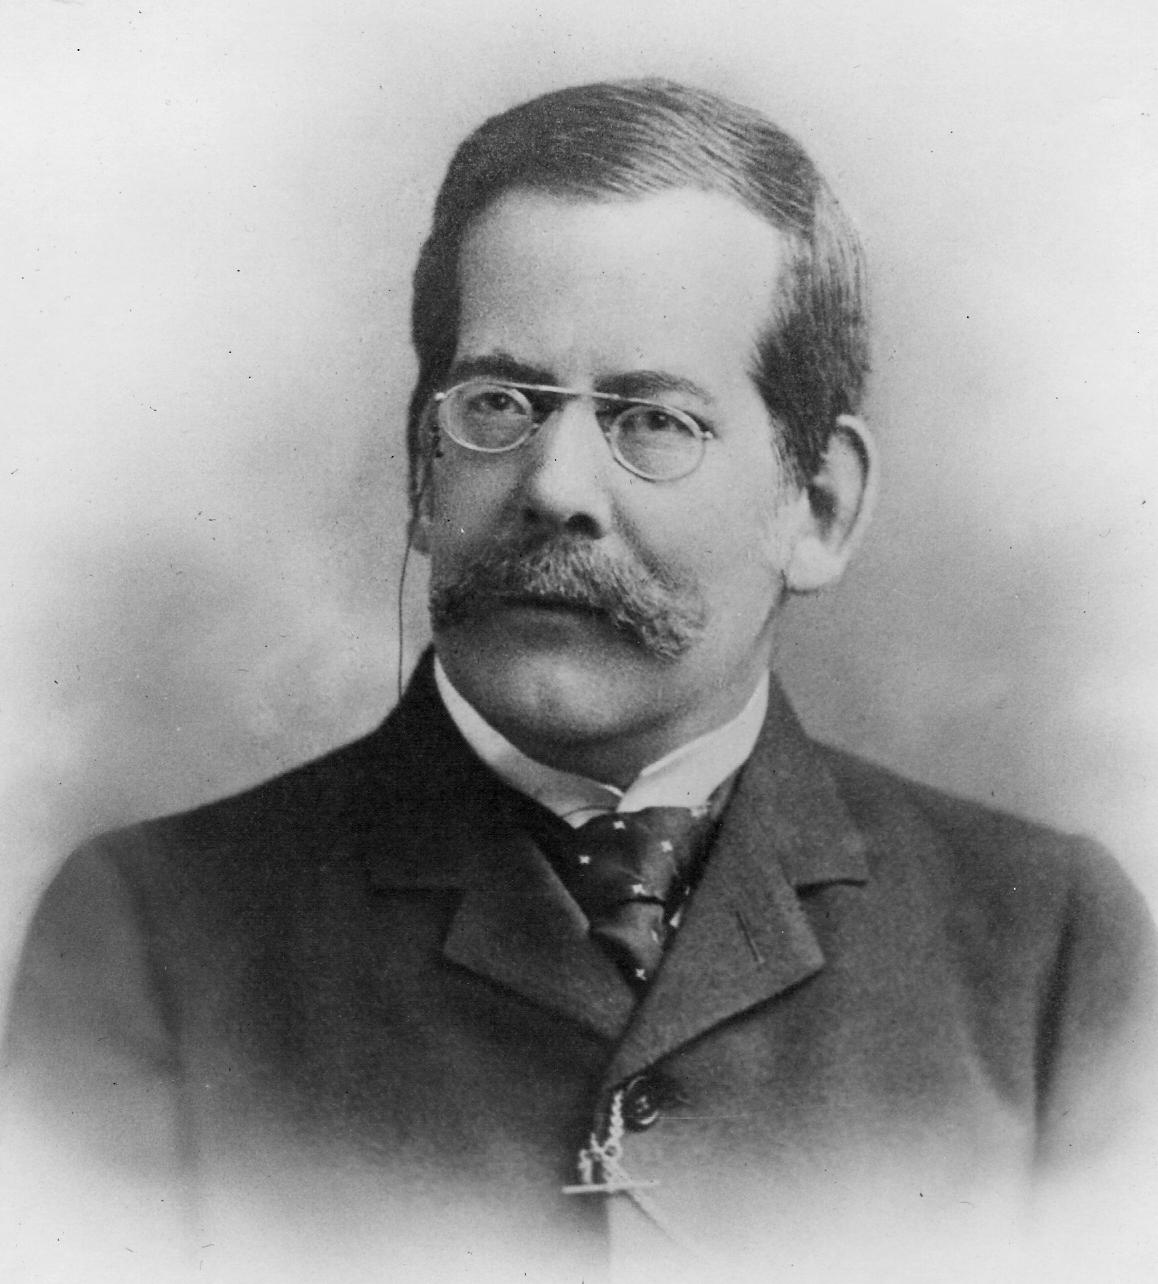
\includegraphics[width=.9\textwidth]{figures/Sweet.jpg}
  \caption{Henry Sweet}
  \label{fig:ch.firth.sweet}
\end{wrapfigure}
Though we could trace the roots of British phonetic research
considerably farther back, a convenient starting point for the present
discussion is the work of \name{Henry}{Sweet}, one of the first in England to
\isi{stress} the scientific status of an inquiry into the facts and
mechanisms of speech. {\Sweet} was born in 1845; after studying various
languages, as well as some {German} philology at the University of
Heidelberg, and spending some time working in an office, he entered
Oxford at the age of twenty-four. While there, he began the series of
studies on the history of \ili{English} (especially \ili{Old English}) which would
establish his reputation as the premier Anglicist of his
day. Unfortunately, his student career at Oxford had a disastrous
conclusion: he was given a fourth-class degree, a result so bad as
hardly ever to be given, and generally reserved for those about whom
the examiners cannot decide whether they are fools or geniuses. This
effectively foreclosed the possibility of a professorial chair at
Oxford, a source of bitterness which became progressively greater to
{\Sweet} throughout his career.

A series of specialized studies, grammars, collections of texts, and
student handbooks devoted to Old and \ili{Middle English} which {\Sweet}
produced between 1869 and 1885 certainly established his stature as a
philologist (though they did not earn him the desired chair in 1876,
1885 or—at his final attempt— in 1901), but it was his work on
phonetics which is of greater interest to us here. This interest was
probably stimulated originally by Alexander Melville
\posscitet{bell67:visible.speech} book \textsl{Visible Speech}, an
attempt to provide a scientific system for recording the facts of
speech in terms of a representation of the articulatory gestures
involved in its production. \posscitet{sweet77:handbook}
\textsl{Handbook of Phonetics} served as the standard reference work
on phonetics in \ili{English} for generations.

Aside from presenting the facts of articulatory phonetics (based
primarily on impressionistic observations), {\Sweet}'s \textsl{Handbook}
is of interest to the modern phonologist in presenting an early
version of {\Saussure}'s `phonemic insight'. {\Sweet} distinguishes clearly
between two related forms of \isi{phonetic transcription}: `Narrow Romic'
and `Broad Romic'. The former, narrow \isi{transcription}, is intended to
present as accurate as possible a representation of all of the facts
relevant to the production of a transcribed utterance which the
phonetician can describe. The \isi{notational system} for Narrow Romic
transcriptions is explicitly intended to be valid
cross-linguistically, and equally apt for the presentation of
utterances in any human language. Broad Romic, in \isi{contrast}, is a
language-particular representation: such a \isi{transcription} should
``indicate only those broader distinctions of sounds which actually
correspond to distinctions of \isi{meaning} in language.'' Though he does not
use the word \isi{phoneme}, {\Sweet} makes it clear that a system of Broad
Romic \isi{transcription} for a given language should provide distinct
symbols only for those elements whose interchange could (potentially)
serve to distinguish words from one another: the \isi{phonemic principle}.

{\Sweet}'s Broad and Narrow Romic transcriptions serve different ends:
the former is practical in intent (since if it is adequately defined,
such a representation provides all of the information necessary to
describe the pronunciation of any transcribed form within a given
language with a minimum of apparatus), while the `scientific' Narrow
Romic was intended to provide ``an accurate analysis of sounds
generally,'' and was thus ``too minute for many practical purposes.''
There is clearly a relation between the two other than their disparate
goals, however: a Broad Romic representation differs from a Narrow one
precisely in omitting mention of those phonetic properties that do not
serve to distinguish meanings. In other words, Broad Romic
\isi{representations} can be regarded as identifying incompletely specified
basic variants, in terms of the discussion in
chapter~\ref{ch.saussure_sound}. These can (in principle) be converted
into fully specified Narrow Romic forms by the addition of
(non-distinctive) phonetic detail.

{\Sweet} thus ranks (along with \name{Jost}{Winteler}, {\DeCourtenay}, and
others) among those who explicitly discussed the fundamental principle
of phonemic analysis well before the publication of {\Saussure}'s
\textsl{Cours}. In fact, it is quite clear when we look into the history of
virtually every tradition in the study of language that transcriptions
which record only those distinctions that serve to distinguish one
word from another within a given language were not only the basis of
the original reduction of languages to writing but were perfectly
familiar in the theoretical study of language as well, rather than the
innovation many writers on \isi{phonemic theory} in the 1930s and 1940s
claimed.

Nonetheless, it would be quite unreasonable to interpret {\Sweet} as a
phonemic theorist in a modern sense, since his concern was exclusively
to devise a practical system of \isi{transcription}. The real innovation in
structuralist \isi{phonemic theory}, beginning with {\Saussure} and
(especially) the Prague school, was the notion that the set of
phonemes (or elements of a Broad Romic representation) in a given
language form a system with an important internal organization. It is
not the notion of a phonemic representation \emph{per se} that sets
off twentieth-century phonology from its phonetically oriented
predecessors but, rather, the conception of this representation as
composed of elements requiring study and analysis in their own
right. `Structuralism' in phonology should not be identified with the
discovery of \isi{phonemic representations}.

{\Sweet} himself published descriptions of the phonetics of a number of
other languages, and beginning in 1885 turned his attention more
toward general linguistics than to his earlier work in \ili{English}. He
supported himself largely through private teaching of \ili{English}, and is
traditionally seen as having served (partially) as the model for
Professor Henry Higgins in Shaw's \emph{Pygmalion} (though according
to \citet{collins.mees99:jones}, the real model for Higgins was
probably \name{Daniel}{Jones}). In 1902, after his final failure to secure a
professorship at Oxford, he was named a Reader in Phonetics there.

To get the university authorities to establish such a position
required him to convince them of the proposition that ``phonology is
not only the indispensable foundation of all philology, but also that
no department, from the highest to the lowest, can be investigated
fully without it, whether it be accidence, syntax, or prosody, or even
that fundamental problem—the origin of language.'' The chair in
comparative philology did not, he argued, provide adequate coverage of
this crucial area, and eventually his rather limited position was
approved. By this time, though, he was so embittered against the
academic establishment that his final years at Oxford were
characterized almost as much by a series of embarrassing incidents
stemming from his feelings of persecution as they were by his actual
accomplishments. He died in 1912.

Though {\Sweet}'s conventional academic career was professionally
disappointing to him, his impact on the study of language in Britain
was enormous. In the period between 1869 and 1885, his influence was
the dominant factor in the principal organization in Britain devoted
to the study of language, the Philological Society; he was president
of the society in 1877 and 1878. As \citet[197f.]{wrenn46:sweet} says,
he ``founded the modern science of phonetics, made it the basis of all
linguistic studies, while at the same time becoming the best
practising phonetician of his age. He provided the first handbooks on
phonetics, the first accurate and scientific recording of the sounds
of living languages in his presentations of Welsh, Swedish, etc., in
the Philological Society's \textsl{Transactions}, and the best
treatments of \ili{English} pronunciation and \isi{orthography} till then
obtainable.'' He also introduced a notion of phonological (as distinct
from purely phonetic) representation, and in general established the
basis for subsequent phonological studies in Britain.

{\Sweet}'s influence thus led to the establishment of phonetics as a
distinct discipline in British universities, especially in connection
with the teaching of languages (both foreign languages and \ili{English} for
foreigners). This development was not limited to Oxford; in 1903 a
series of evening lectures began at University College, London, on
phonetics as applied to \ili{French}, and other lectures were given there on
general phonetics with special reference to \ili{English} and \ili{German}. In
1907, a new lecturer was appointed at University College in the area
of phonetics, \name{Daniel}{Jones}. It was largely through his efforts that
the `London School of Phonetics' grew and prospered in the coming
years.

\begin{wrapfigure}{r}{.35\textwidth}
  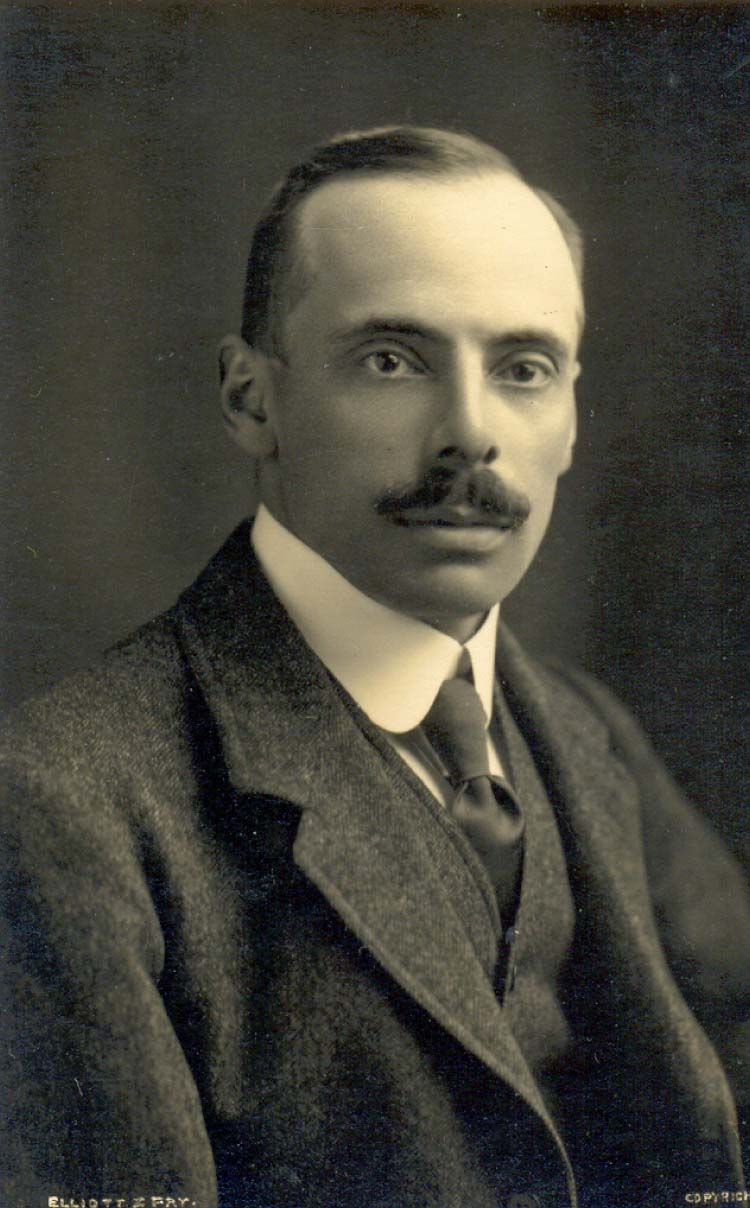
\includegraphics[width=.9\textwidth]{figures/Daniel_Jones.jpg}
  \caption{Daniel Jones}
  \label{fig:ch.firth.jones1}
\end{wrapfigure}
Daniel {\Jones} was born in 1881 in London.\footnote{A comprehensive account of
  \name{Daniel}{Jones}' life and work is provided by
  \citet{collins.mees99:jones}.} During his school years, he studied a
number of languages, though his Cambridge B.A. was a somewhat
undistinguished one in \isi{mathematics}. His father had pressed him to
study law, and he did earn an M. A. in this, but never practiced as a
lawyer. In 1900 he studied \ili{German} phonetics at Marburg with \name{William}{Tilly} and, in 1905-6, \ili{French} phonetics with \name{Paul}{Passy} in Paris. {\Passy}
was almost literally a father figure to him: he married {\Passy}'s
daughter, and it was through {\Passy}'s influence that he was asked to
lecture at University College at the beginning of 1907. He was offered
a \isi{regular} appointment later that year (shortly after completing his
law degree and being admitted to the Bar). Over the ensuing years, he
built his lectureship into a substantial department of phonetics. He
was also a major force, together with {\Passy}, in the International
Phonetic Association, and served as co-editor (later sole editor) of\textsl{ Le
maître phonétique} for much of his career. His London appointment was
upgraded to the status of a reader in 1914, and he was made professor
in 1921. He continued to teach and direct the department at University
College until 1949; after his retirement, he pursued his research as
professor emeritus until his death at the age of eighty-six in 1967.

{\Passy} and {\Sweet} were undoubtedly the major influences on {\Jones}'s early
career, but in 1911 he came into contact with {\Ščerba}, who discussed
with him {\DeCourtenay}'s notion of the \isi{phoneme} (at least as it
had been taught in his later St. Petersburg years; see
chapter~\ref{ch.kazan} above). Another of {\Baudouin}'s students, 
\name{Tytus}{Benni} from Warsaw, provided {\Jones} with a more extensive opportunity to
discuss these ideas two years later. ``The immense importance of the
theory then became very clear to me, especially in its relation to the
construction of phonetic transcriptions, to the devising of alphabets
for languages hitherto unwritten, and in general to the practical
teaching of foreign spoken languages. Consequently by about 1915 the
theory began to find a {regular} place in the teaching given in the
Department of Phonetics at University College''
\citep[6]{jones57:meaning.of.phoneme}.

The {stress} on practical applications of the notion of phonemic
representation in this remark is entirely characteristic of {\Jones}'s
attitude, as it had been for {\Sweet} (and Passy, who also urged students
of language to ``ne noter dans les textes que les différences
significatives''—in order not to ``rendre les textes phonétiques
illisibles''). {\Jones} goes well beyond {\Sweet} in developing an
articulated notion of the \isi{phoneme} as a basic constituent in a theory
of language (see especially \citealt{jones50:phoneme}), but the
motivation for his theoretical choices is always practical rather than
one deriving from general scientific considerations.

This is particularly clear in his discussion of the definitional basis
of the pho\-neme. {\Jones} observes that at least two different
conceptions of the \isi{phoneme} can be distinguished. On the one hand,
phonemes can be thought of as psychological constructs, ``a
speech-sound pictured in one's mind and `aimed at' in the process of
talking'' \citep[7]{jones57:meaning.of.phoneme}. This picture, a
version of the `\isi{fully specified basic variant} view' identified in
chapter~\ref{ch.saussure_sound} above, {\Jones} correctly attributes to
{\Baudouin}. On the other hand, ``viewed from the `physical' angle a
\isi{phoneme} is a family of uttered sounds (segmental elements of speech)
in a particular language which count for practical purposes as if they
were one and the same'' (\emph{Ibid.}). We will return below to the
precise content of this view, but it is fairly clear that it is
distinct from the psychological conception introduced above.

The remarkable thing about {\Jones}'s discussion of the choice between
these two ways of founding the {concept} of the \isi{phoneme} is that in a
number of places he expresses a preference for the `psychological'
view, finding it conceptually superior, yet he consistently opts for
the `physical' definition on practical grounds. ``When it became
necessary for me to come to a decision between the two, I found it in
the end impossible to escape the conclusion that the physical view of
the \isi{phoneme} is on the whole better suited to the needs of ordinary
teaching of spoken languages and (in spite of {\Sapir}'s experiences) for
those who are called upon to reduce to writing languages hitherto
unwritten or to improve on existing unsatisfactory orthographies. I
find the physical view more easily comprehensible to the ordinary
student of languages than any other''
\citep[9]{jones57:meaning.of.phoneme}. This concern for considerations
relevant to the design of orthographies recalls the work in America of
Kenneth \citet{pike47:phonemics}, a book which bears the subtitle
\textsl{A Technique for Reducing Languages to Writing}.

\begin{wrapfigure}{r}{.35\textwidth}
  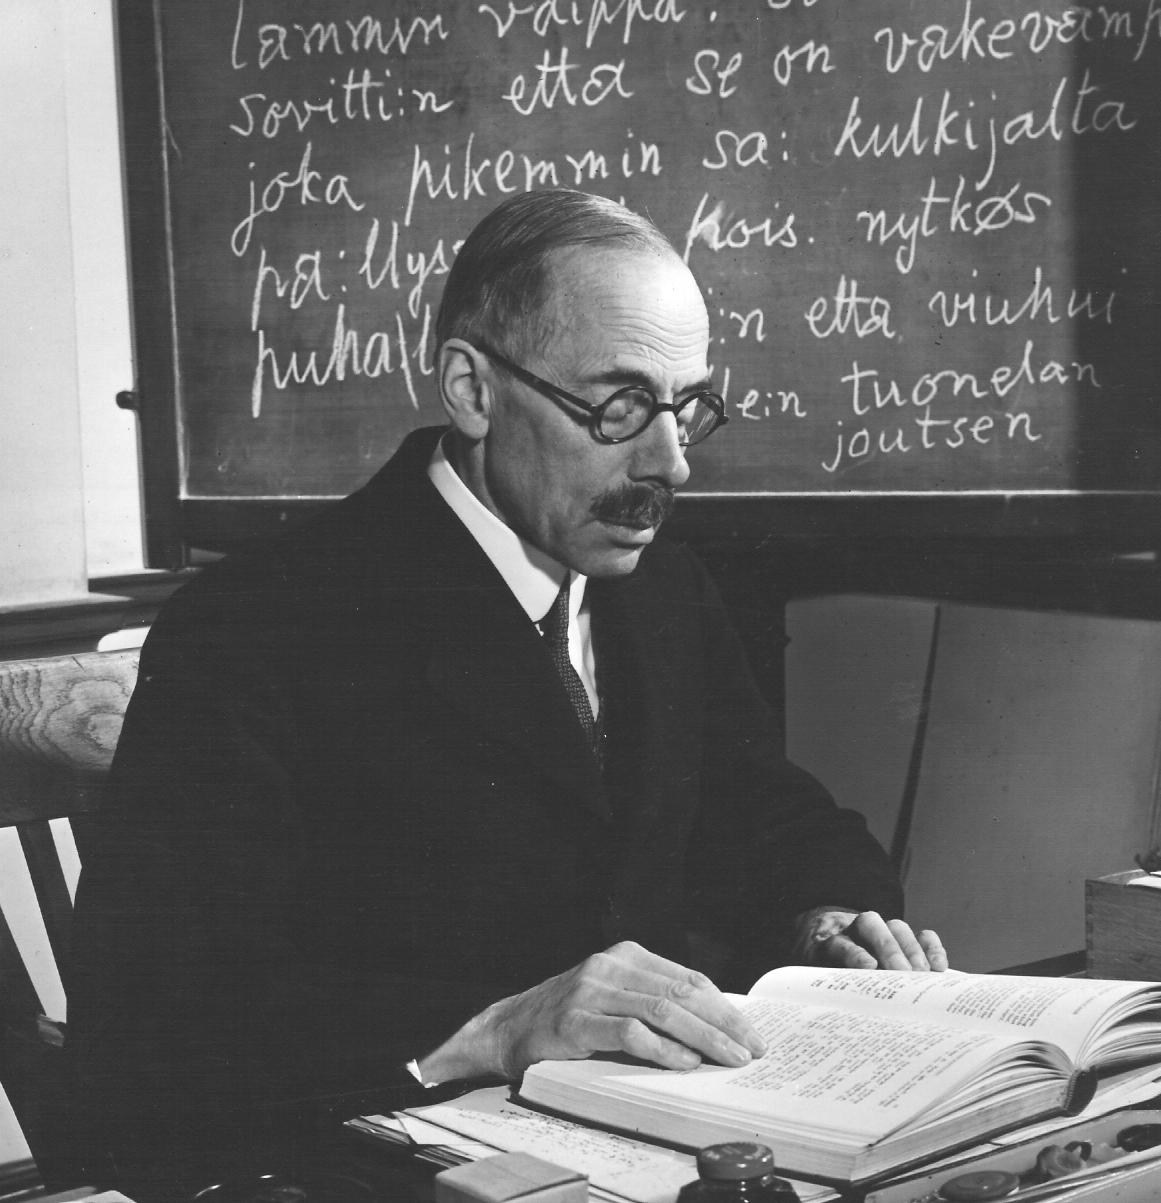
\includegraphics[width=.9\textwidth]{figures/jones_daniel.jpg}
  \caption{Daniel Jones}
  \label{fig:ch.firth.jones2}
\end{wrapfigure}
In fact, {\Jones}'s physicalist view of the \isi{phoneme} cannot be equated
with any of the pictures presented in chapter~\ref{ch.saussure_sound}
above. Over a number of years (starting in the 1920s) he
refined the definition referred to above, arriving (in
\citealt{jones50:phoneme}, as quoted in
\citealt[14]{jones57:meaning.of.phoneme}) at the conception of a
\isi{phoneme} as ``a family of sounds in a given language which are related
in character and are used in such a way that no member ever occurs in
a word in the same phonetic context as any other member'' as a
definition which is ``as precise as words can make it''
\citep[14]{jones57:meaning.of.phoneme}. A \isi{phoneme} on this view, then,
is not itself a sound (either completely or partially specified,
physical or psychological) but, rather, the name of a \emph{set} or
\emph{family} of sounds. This view is a physical one in the sense that
the individual members (or, as they were called in American practice,
\emph{allophones}) of a \isi{phoneme} are concrete, fully specified
sounds—but the \isi{phoneme} itself, as the name of a set, is an abstraction
of a higher level.

Notice that the stated basis for including different sounds in the same
\isi{phoneme} is not their failure to distinguish meanings of words. It is
the fact that they never occur in the same phonetic environment: in
other words, that they are in \isi{complementary distribution} (American
terminology which {\Jones} explicitly accepts, though he does not use
it). This was not by any means an accident, but a reflection of
{\Jones}'s belief that ``any reference to \isi{meaning} is out of place in a
physical definition of the \isi{phoneme}. It is incumbent on us to
distinguish between what phonemes \emph{are} and what they
\emph{do}. \textbf{Phonemes} \emph{are} \textbf{what is stated in the
  definition. What they} \emph{do} \textbf{is to distinguish words
  from one another}'' (\citealt[15]{jones57:meaning.of.phoneme};
emphases in the original). The elimination of \isi{meaning} from the
definition thus does not follow (as it would for American
structuralist phonemicists—see chapter~\ref{ch.structuralists}) from a
general rejection of \isi{meaning} as a valid linguistic category; rather,
it results from considerations of conceptual clarity.

{\Jones}'s work involved the study of a wide variety of languages: he
wrote book-length descriptive studies of languages as diverse as
\ili{Cantonese} \citep{jones12:cantonese}, \ili{Sechuana}
\citep{jones16:sechuana}, \ili{Sinhalese} \citep{jones19:sinhala}, and
\ili{Russian} \citep{jones23:russian}, as well as descriptions of \ili{English}
pronunciation that can still claim to be in their way definitive. His
theory of phonological structure, however, is clearly limited to a
particular (practically oriented) view of the nature of phonological
\isi{representations}. Regularities of relationship among forms do not enter
significantly into this picture, which is founded entirely on the
notion of segment-sized phonemes as the fundamental units of
linguistic \isi{sound structure}.


\begin{wrapfigure}{r}{.5\textwidth}
  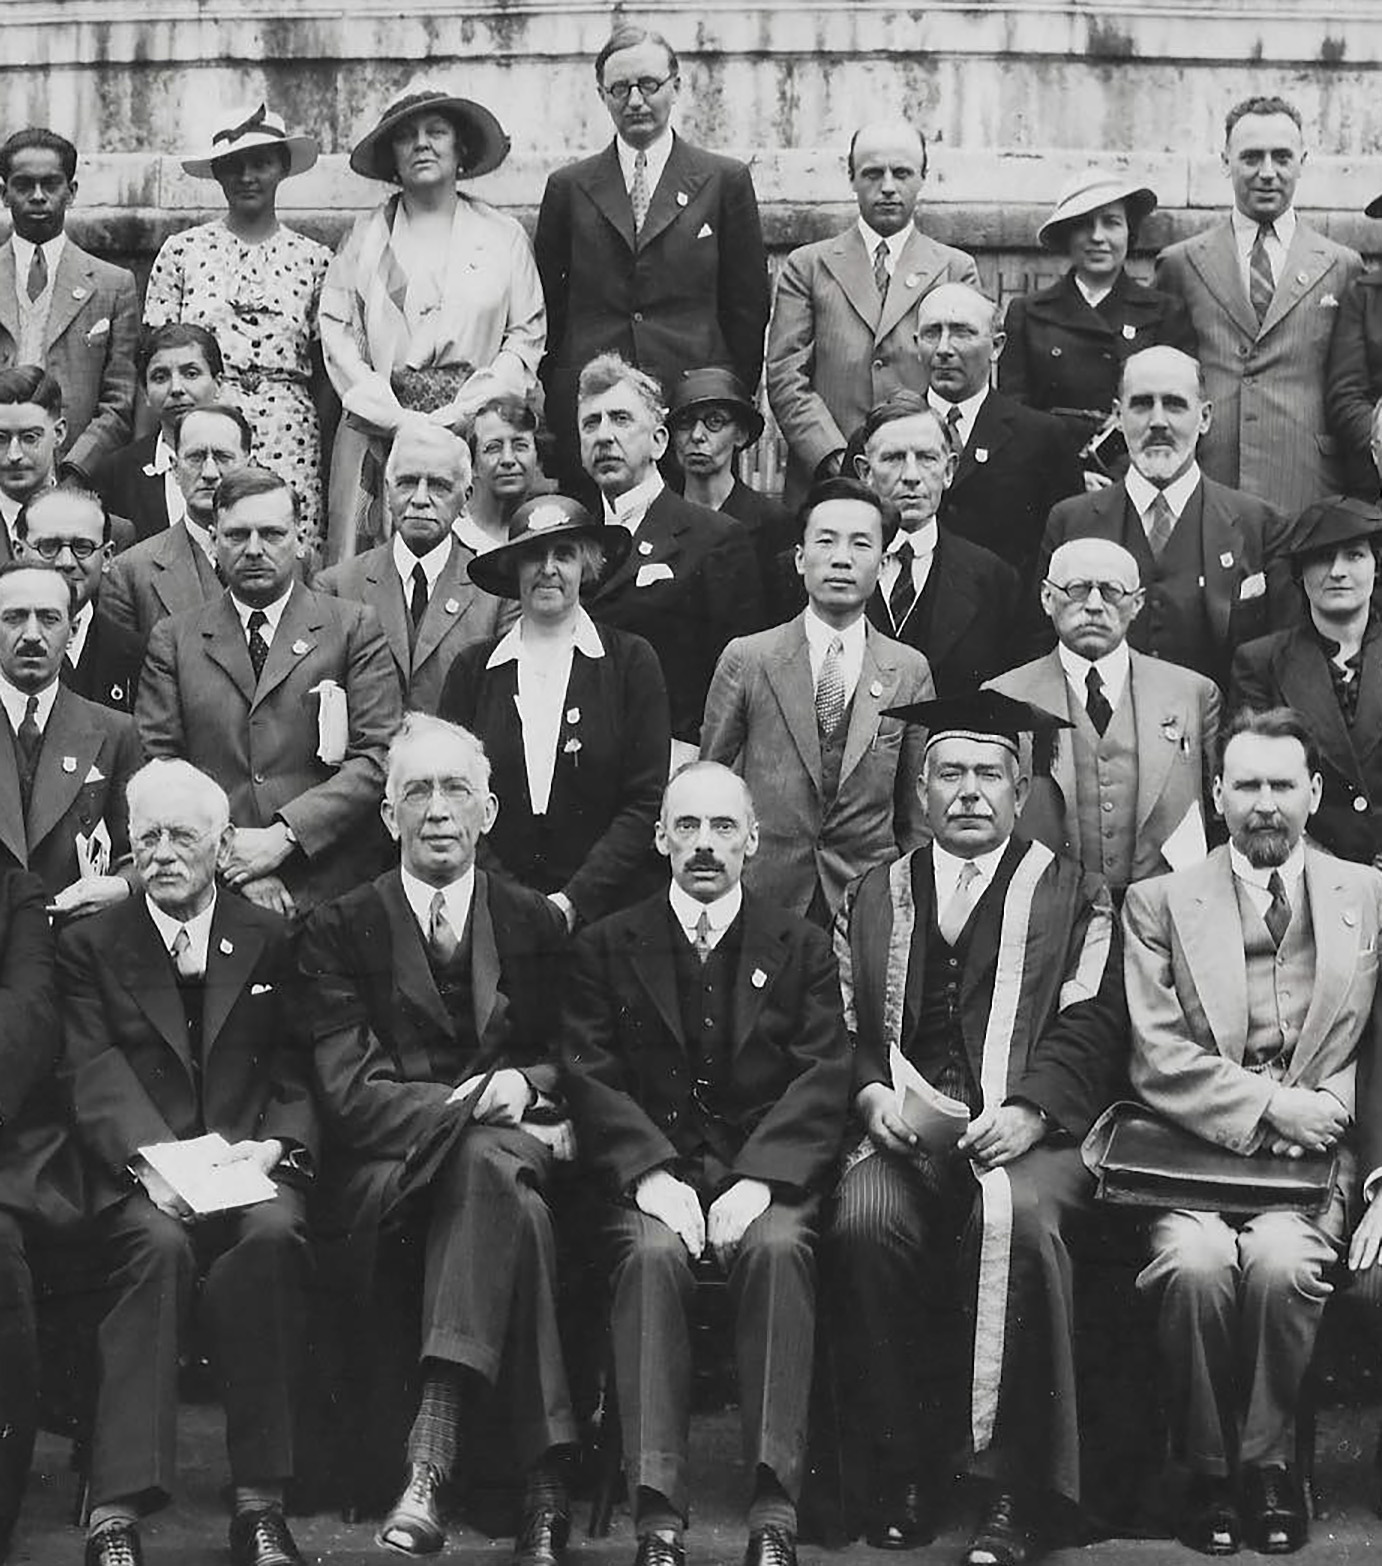
\includegraphics[width=.9\textwidth]{figures/ICPhS_1935.jpg}
  \caption{From the 1935 London ICPhS: Louis Hjelmslev (standing, top
    middle); Otto Jespersen (seated, left); Daniel Jones (seated,
    middle); Nikolai Trubetzkoy (seated, right); J. R. Firth (standing, behind
    Jespersen)}
  \label{fig:ch.firth.icphs_1935}
\end{wrapfigure}
Much of the theoretical apparatus of \posscitet{jones50:phoneme}
\textsl{The Phoneme} is devoted to clarifying the basic properties of
the object of study in linguistics. He believed that a coherent
analysis can only result from the study of phonological properties of
(isolated) words, in the speech of individual speakers within a
uniform speech style, and developed a set of terms (\emph{\isi{variphone}},
\emph{\isi{diaphone}}, and others) to support this conception. 
He was also
concerned to reserve the word \emph{\isi{phoneme}} for standard segmental
units, and proposed (in \isi{contrast} with much American usage) the terms
\emph{\isi{toneme}}, \emph{\isi{chroneme}}, and \emph{\isi{stroneme}} to refer to
distinctive units of \isi{tone}, length, and \isi{stress} respectively. The
resulting theory is one that, whatever its practical merits in
relation to language teaching and orthographic design, still addresses
only a very limited range of the general issues involved in the study
of \isi{sound structure}.

However noteworthy the contributions of {\Sweet}, {\Jones}, and their
students to phonetic research, they do not fall far outside the
mainstream of thinking about the nature of sounds and their relations,
languages and their sound patterns. There are therefore few features
of their views on strictly phonological topics which would warrant
close independent attention in a work such as the present one. If
British linguistics in the twentieth century has a clearly distinctive
position vis-à-vis all other schools of phonology, this is largely due
to the work of {\Jones}' successor at the center of Linguistics in
London, \name{John Rupert}{Firth}.

\begin{figure}
  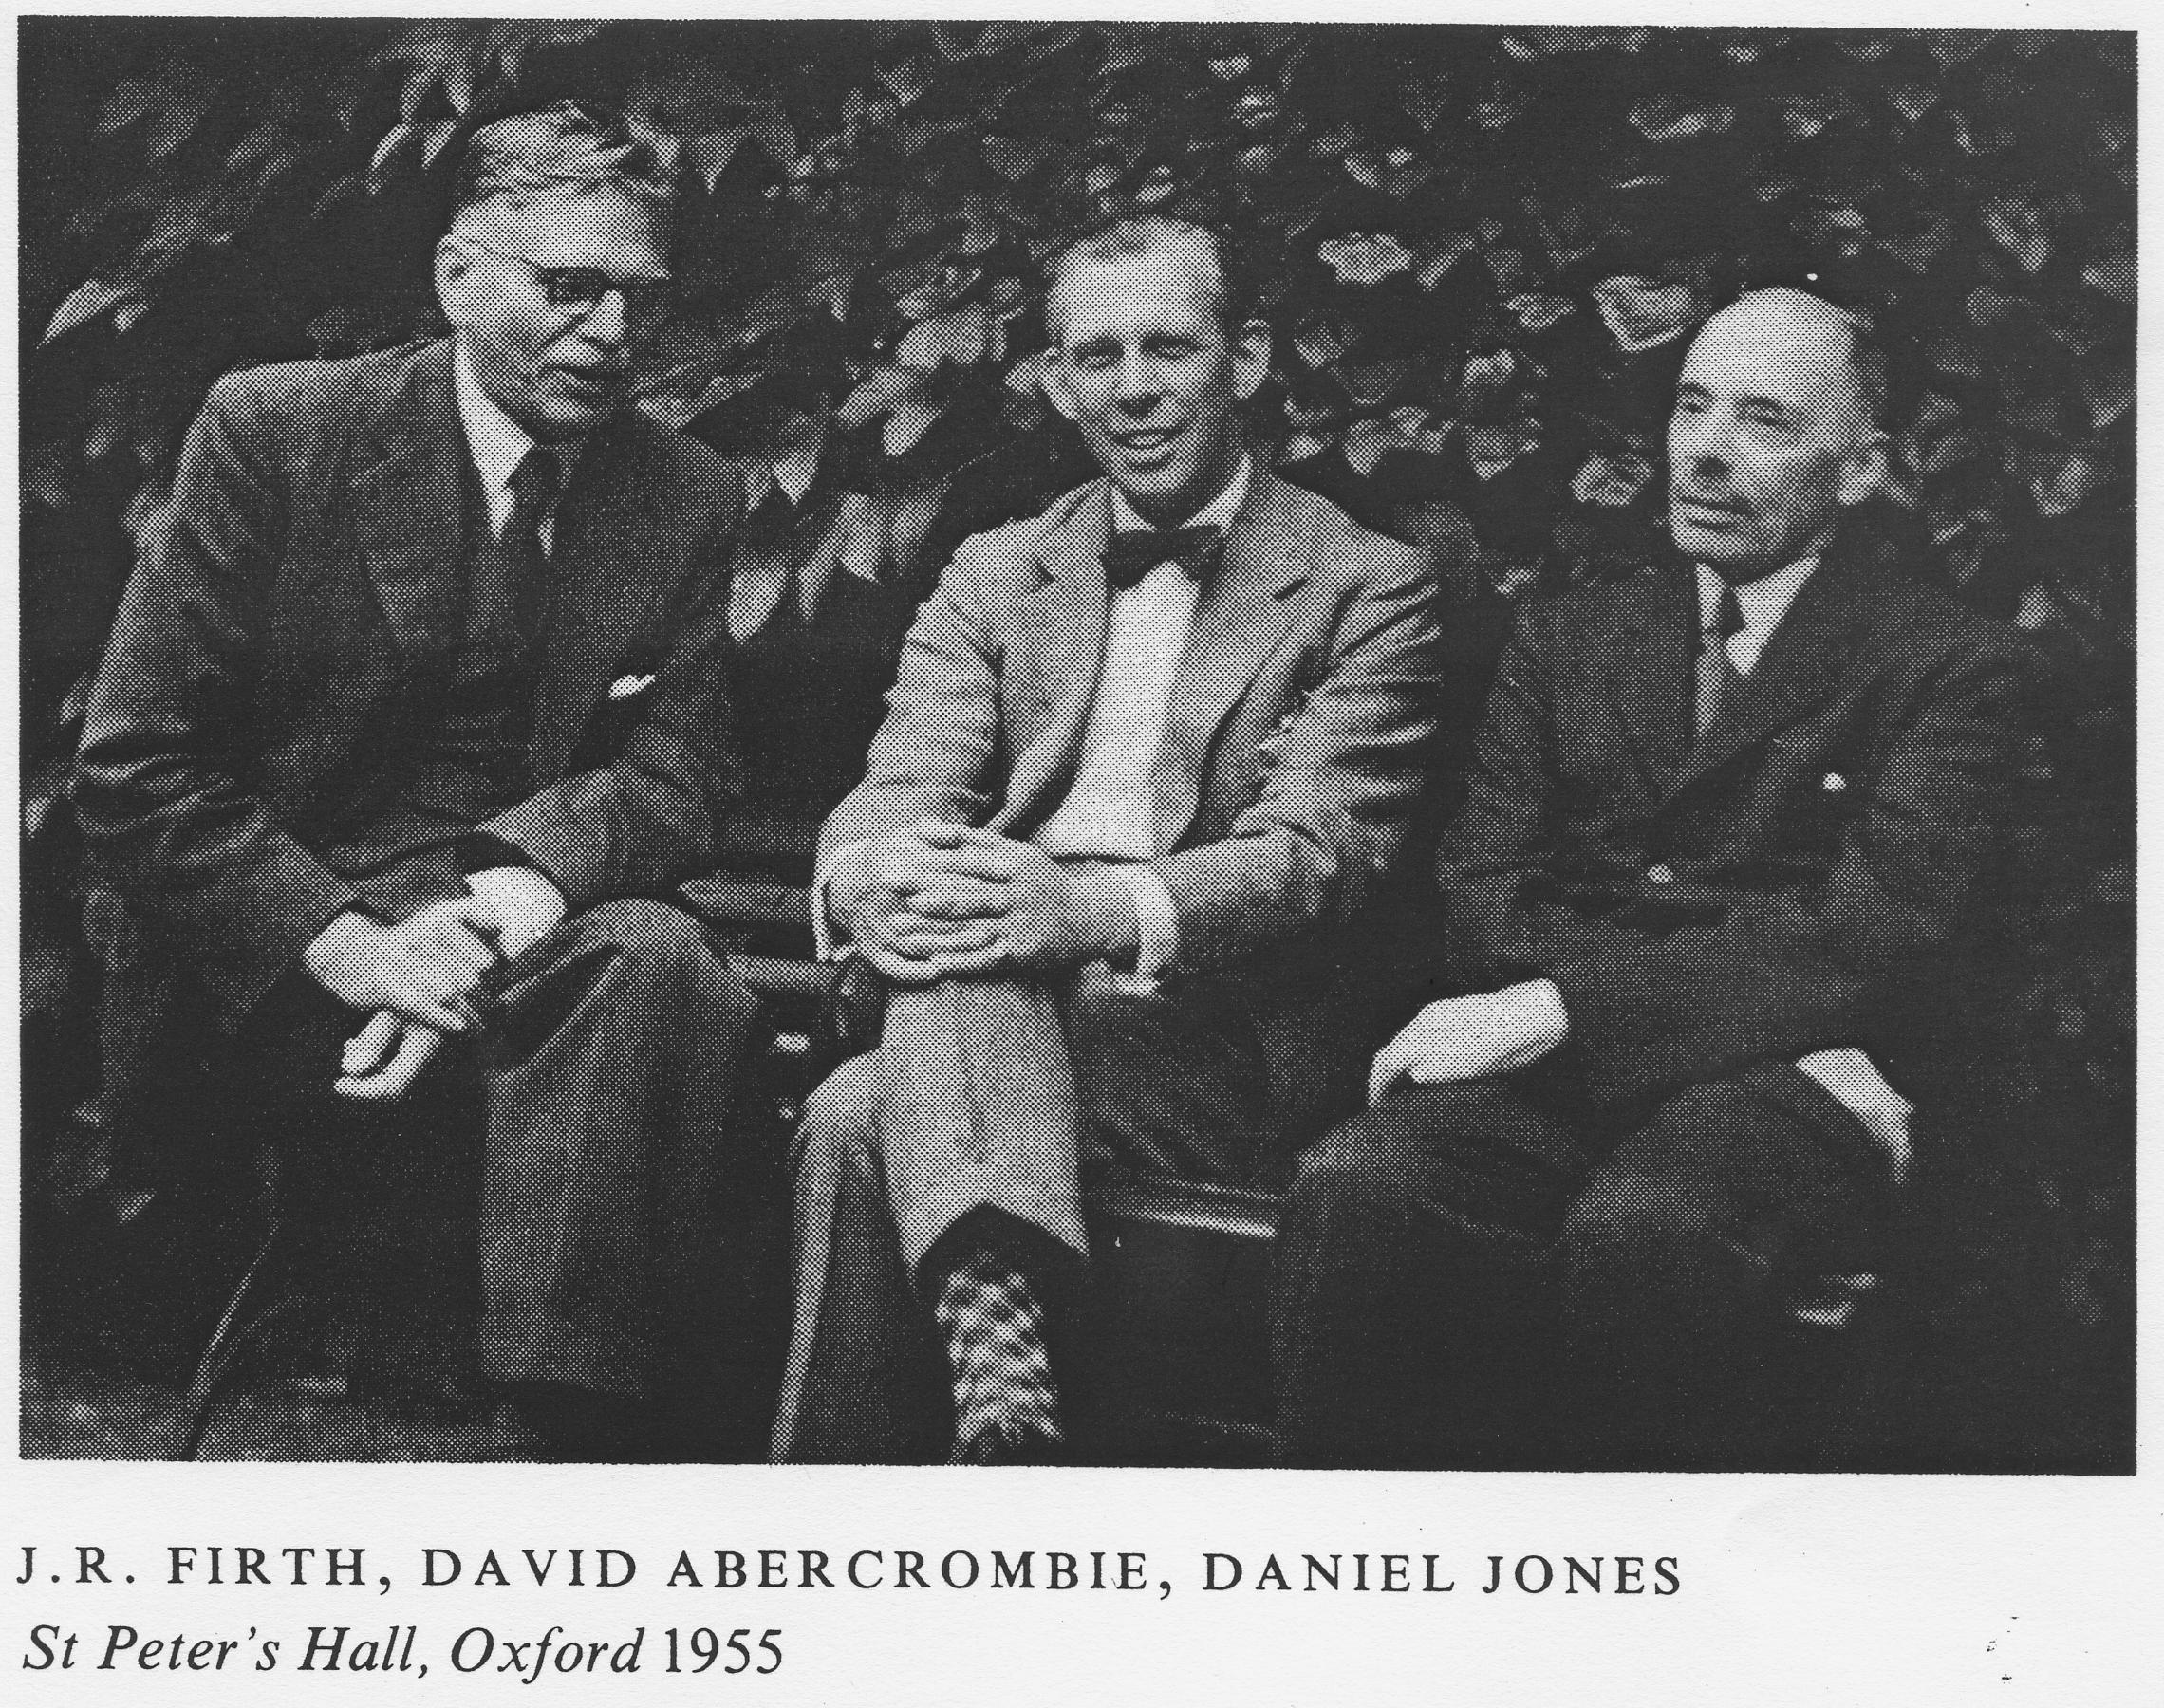
\includegraphics[width=.7\textwidth]{figures/Firth-Abercrombie-Jones-1955.jpg}
  \caption{}
  \label{fig:ch.firth:firth-abercrombie-jones}
\end{figure}


\section{J. R. Firth's life}


{\Firth} was born in Keighley, Yorkshire in 1890, and spent his early
years in that area. \footnote{A detailed account of {\Firth}'s life and
  career based on extensive study of archival material is provided by
  \citet{plug08:firth.bio}. Some of the details below are cited from
  that source.} In 1908 he began the study of history at Leeds
University, and graduated in 1911 with a first-class honours BA. He
continued with some teacher training and an MA, and briefly taught
history in Leeds. His ambition at that point was to become a Professor
of History in India or the British colonies, and he applied for such a
post in Amritsar through the Indian Educational Service. Nothing came
of this, or of subsequent applications of the same nature, but in 1914
he was offered a post as Master of the Training Class for Teachers in
European Schools, Sanawar, the Punjab. This was not a position in
history, but he accepted it in any event, and moved to Sanawar.

Here he was in charge of the college where Indian students were
trained in \ili{English} to teach a variety of subjects. He soon became
frustrated by the low standard of training in \ili{English} for these
students, an issue that led to his later concerns both for teaching
methods in \ili{English} and for practical phonetic training. Not long after
arriving in the Punjab, however, he was called up into the British
army, and spent the years until 1919 serving in East Africa, India and
Afghanistan. Upon his return, the Indian Educational Service appointed
him as Professor {English} at the University of the Punjab in Lahore,
apparently without consulting him.

In Lahore, he was primarily occupied teaching \ili{English} phonetics and
grammar. During this period he became interested in the phonetics of
Indian languages, in the Indian grammatical tradition, and in the
literature of general linguistics as it was developing at the time,
especially {\Saussure}'s \textsl{Cours}. A study leave in 1923-24 allowed
him to visit a variety of centers of activity in linguistics in
France, Switzerland, the Netherlands, and Scandinavia, with the stated
goal of studying phonetics and methods of teaching \ili{English}, but also
with the intention of learning more about general linguistics.

He also spent two terms as a student in \name{Daniel}{Jones}' Department of
Phonetics at University College, London. While there, he participated
in ear training sessions led by \name{Arthur}{Lloyd James}. {\LloydJames} was
sufficiently impressed with {\Firth}'s abilities that when he left UCL for
the School of Oriental Studies in 1926, he recommended to {\Jones} that
{\Firth} be appointed as his replacement. {\Jones} offered him a position as
Senior Assistant, which he took up in October, but shortly afterwards
resigned and returned to Lahore, saying he would return in 1929. In
fact, though, he was able to return to London in 1928, and {\Jones} (who
was eager to have him back) offered him a position as Senior
Lecturer--an improvement in title, though with no significant
consequences for his salary.

{\Firth}'s relations with {\Jones}, though always perfectly correct, were
never particularly cordial, on the basis both of personal style and
{\Firth}'s discomfort with {\Jones}' view of phonological structure. This
led to a certain degree of tension with the Department of Phonetics at
UCL, and ultimately to a parting of their ways which seems to have
been welcomed by both.  Although he remained on the staff of {\Jones}'s
department through 1938, he was increasingly occupied with part-time
positions elsewhere as well. He served as assistant in the sociology
of languages at the London School of Economics and Political Science;
in the early 1930s, he participated in a series of seminars there with
the anthropologist \name{Bronisław}{Malinowski}, which had an important effect
on his general view of language. He also served as special lecturer in
the phonetics of Indian languages at the Indian Institute in Oxford.

London University's School of Oriental Studies (renamed in 1938 as the
School of Oriental and African Studies, largely as a result of the
important work done there on African languages by linguists such as
\name{Ida}{Ward}) had long been involved in work on language, and {\Firth} was
happy to move there definitively from UCL. After a year spent in India
working on Gujarati and Telugu, {\Firth} became a full-time senior
lecturer in linguistics and Indian phonetics in the Department of
Phonetics and Linguistics at SOAS in 1938. As with his appointment at
UCL, this came at the recommendation of {\LloydJames}, now Head of the
Department of Linguistics and Phonetics at the School.  In 1940, {\Firth}
was appointed to the position of reader, and in 1941 he succeeded
{\LloydJames} as Head of the Department on the latter's
retirement.\footnote{There is a tragic story here. In 1941, Arthur
  {\LloydJames} was convicted of killing his wife, the violinist \name{Elsie
  Winifred}{Owen}, apparently out of concern that the war would
  otherwise cause her hardship. He was found insane, and committed to
  the Broadmoor Criminal Lunatic Asylum, where he committed suicide in
  1943.}

During World War II, {\Firth}'s department rapidly grew from a staff of
two to fourteen, largely as a consequence of the responsibilities it
undertook in the teaching of Oriental languages (particularly
\ili{Japanese}). This development was in stark {contrast} to that of Daniel
{\Jones}'s department of phonetics at University College, which ``after
1939 \ldots\ was of necessity greatly reduced in staff and output of
work'' \citep{jones48:london.school}. While ``in the autumn of 1943 it
was found possible to recommence courses on a limited scale''
(\emph{Ibid}.), {\Jones}'s department had clearly been eclipsed in
importance by {\Firth}'s department at SOAS. It is interesting to compare
this effect of wartime language-teaching work on linguistics in
Britain with the effect the army language program had in stimulating
and consolidating the position of the `neo-Bloomfieldian' linguists in
the United States (see chapter~\ref{ch.structuralists} below).

\begin{wrapfigure}{r}{.4\textwidth}
  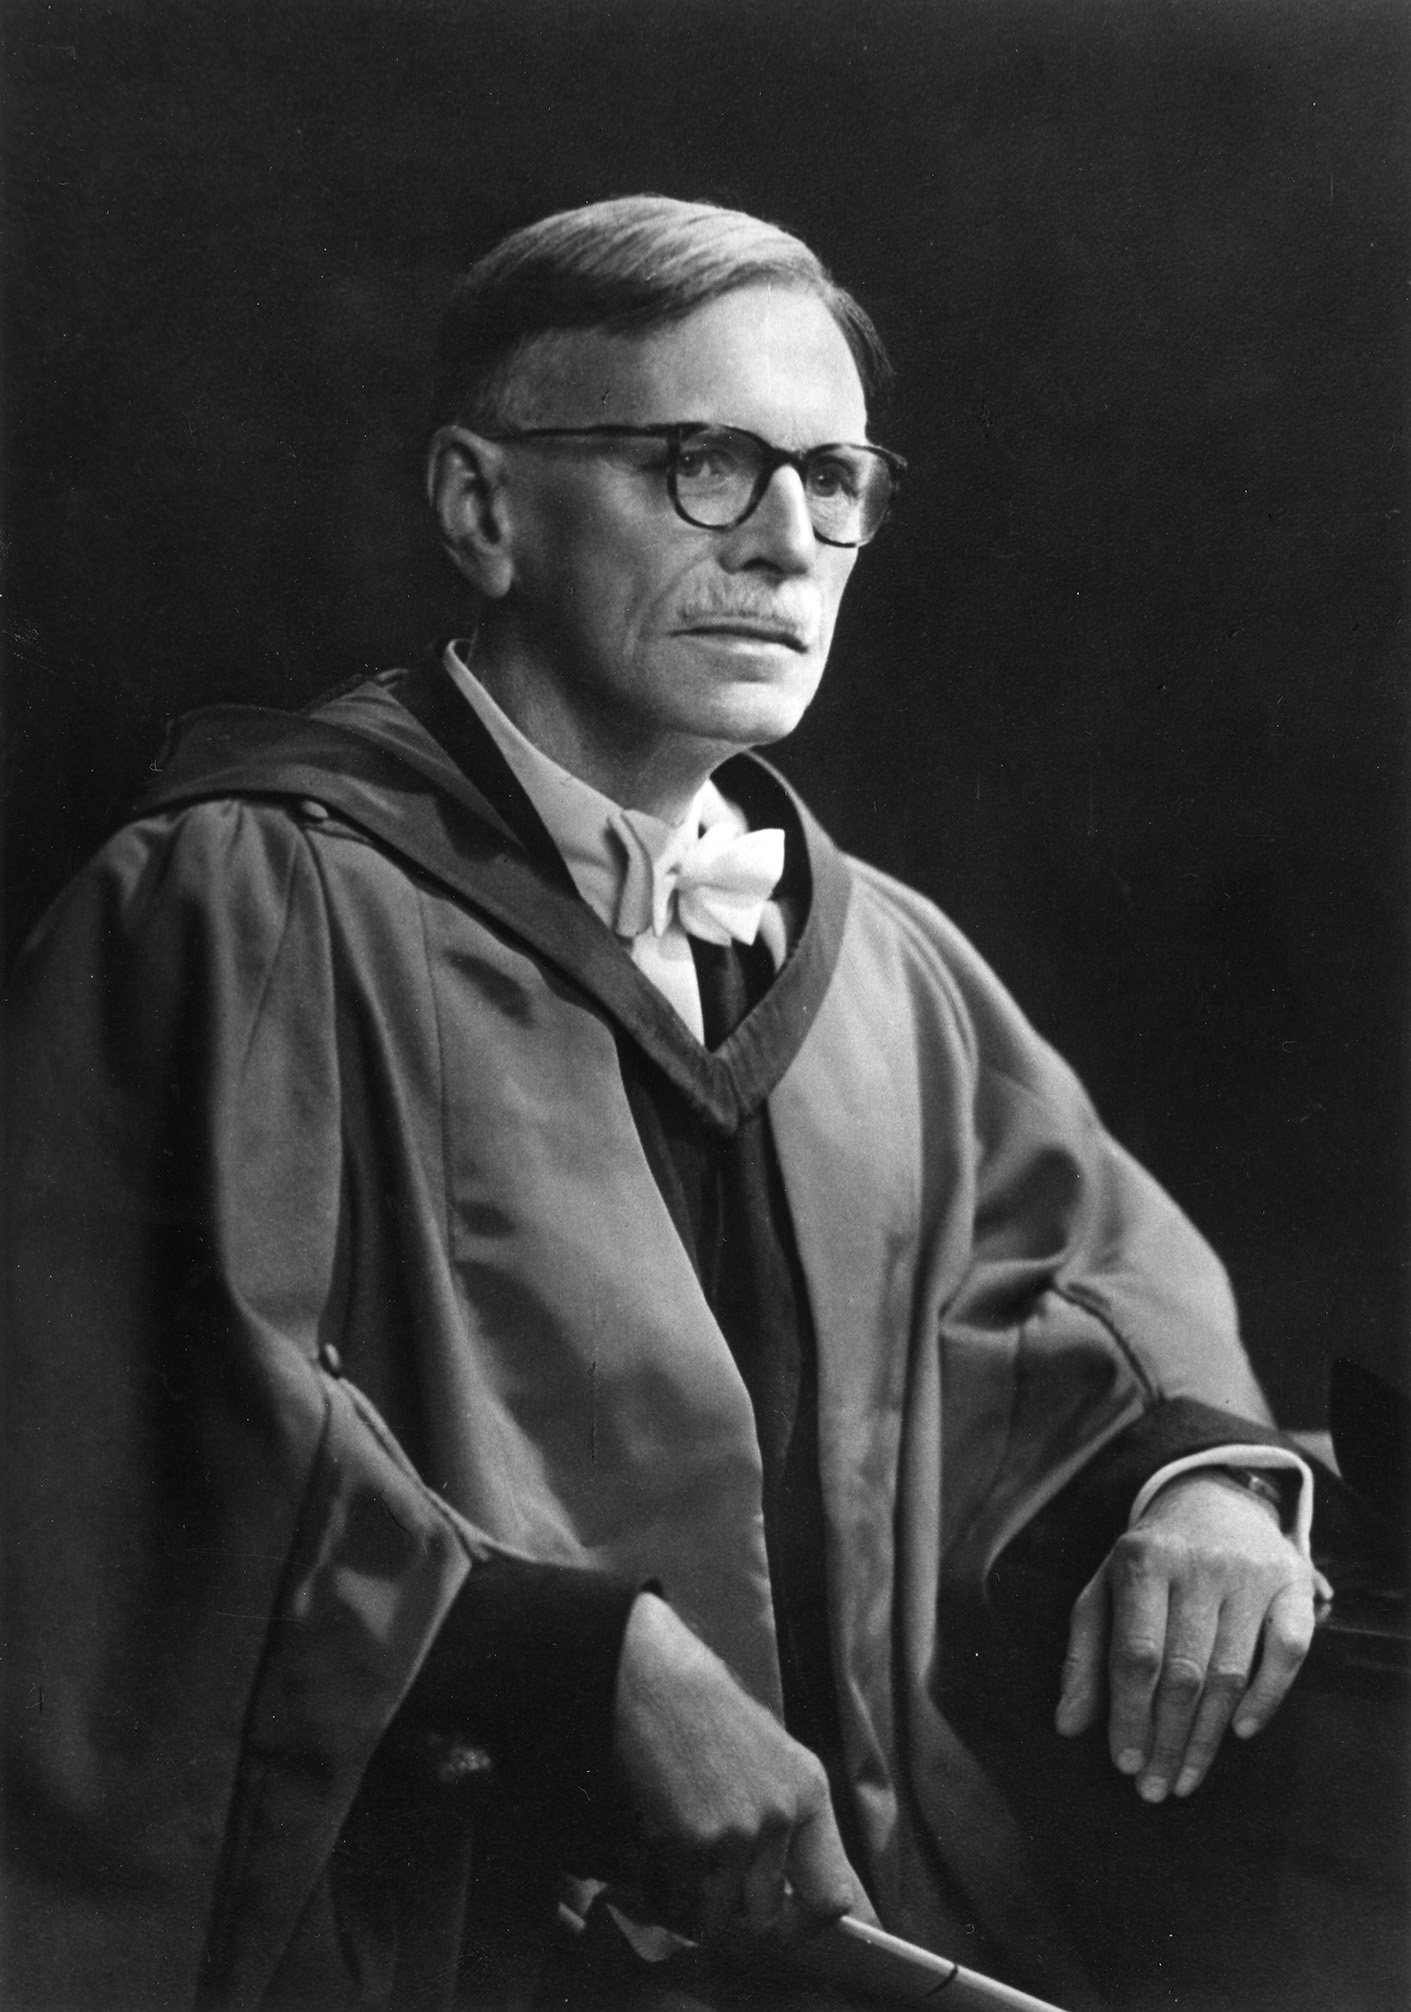
\includegraphics[width=.9\textwidth]{figures/firth_soas.jpg}
  \caption{John Rupert Firth}
  \label{fig:ch.firth.firth_soas}
\end{wrapfigure}
In 1944, the first chair of general linguistics in Britain was
established at the School of Oriental and African Studies, and {\Firth}
was named to it. This position served as the basis for the general
extension of his influence in British linguistics and phonetics until
his retirement in 1956. In at least two areas, phonology and
semantics, his thought had developed into distinctive and novel
theories, which became the central topics of discussion during this
period (and subsequently) among British linguists.

In phonology, \posscitet{firth48:sounds:prosodies} paper ``Sounds and
Prosodies'' served to indicate, if hardly to codify, the characteristic
features of a position radically at odds with any theory of sound
structure (such as that of \name{Daniel}{Jones}) that is based centrally on
the \isi{phoneme}. Opinion varies as to whether the development of prosodic
analysis should be dated from this paper or from some of {\Firth}'s
earlier work such as \citet{firth.rogers37:hunanese}. It is fairly
clear, though, that although there is substantial continuity between
the views expressed in \citealt{firth48:sounds:prosodies} and that of
{\Firth}'s work in the middle and late 1930s, much of the development of
\isi{prosodic analysis} in its application and as a distinctive theory was
the result of work by {\Firth}'s colleagues in later years
\citep{coleman04:firth.1930s,battaner-moro06:firth.1930s}.

Although his engagement with international scholarly interchange is
not significantly reflected in his published work
\citep[369]{plug08:firth.bio}, {\Firth} was certainly not unaware of
linguistic work outside of Britain. He refers to ``several
opportunities of exchanging views with colleagues of the {Prague School}
and other European linguists'' \citep{firth35:distribution}; he had met
{\Trubetzkoy} on the occasion of visits to London by the latter in the
1930s ({\Trubetzkoy} described {\Firth} to {\Jakobson} in a letter after the
1935 London Congress as the only scholar he had met in Britain who
could be called a linguist in the sense he and {\Jakobson} had of the
field). While he had little interest in {\Hjelmslev}'s work, he refers to
it occasionally (if only to reject its significance) and was evidently
familiar with it. He taught in the 1948 \isi{Linguistic Institute} at the
University of Michigan, and refers often enough to American work to
show that he was acquainted with its main themes.

He devoted considerable energy to the study of the history of
linguistics, and \citet{firth46:english.school}, ``The {English} School
of Phonetics'', provides evidence for the substantial accomplishments
of {English} phoneticians well before the rise of comparative
\ili{Indo-European} philology in Germany. In a \citeyear{firth49:atlantic}
paper, he discusses the relation between British and American
linguistics—but devotes much of his attention to eighteenth-century
writings on language by \name{Benjamin}{Franklin}, \name{Noah}{Webster}, and \name{Lindley}{Murray}. {\Firth} clearly saw {\Sweet} as his major inspiration in the
earlier tradition; he certainly shared with {\Sweet} at least a
caustic attitude toward {German} scholarship, though it is hard to find
substantial points of comparison between them. Despite his
acquaintance both with the history of the field and with contemporary
work in linguistics being done outside Britain, {\Firth}'s own
theoretical position remained essentially \textit{sui generis}.

{\Firth}'s writings on general linguistics (and on phonology in
particular) are nearly Delphic in character. Even the papers one might
most expect to present systematic expositions of his theoretical
position, such as \citealt{firth48:sounds:prosodies,firth57:synopsis},
are full of obscure and allusive references and completely unclear on
essential points. His students were perfectly aware of this
characteristic of his writing: indeed, they often seem to take a
perverse pride in {\Firth}'s very lack of clarity.

{\Firth}'s influence can hardly be attributed to his published work, much
of which is collected as \citet{firth57:papers} and
\citet{palmer68:firth.papers}. Nonetheless, while this work does not
come close to presenting a unified theory of linguistics (or even of
some part of it, such as phonology), it is clear that he did at a
minimum inspire the formation of a distinct position among his
students. Although it would be a mistake to suggest that this
represented a closed, definitive theory, one could plausibly ask what
important and vital theoretical position ever attains to such a
finished status. Certainly the papers represented in such volumes as
\citet{studies.in.linguistic.analysis} and \citet{palmer70:prosodic}
represent as much of a substantive consensus as would be found in
comparable collections of work within any other theoretical framework
in twentieth-century linguistics.

{\Firth} and his coworkers were obviously in substantial agreement about
the goals, methods, and principles of a particular approach to
phonological analysis; and it is an interesting problem to determine
just how this picture emerged. We have very little evidence for the
actual character or modality of {\Firth}'s influence on his
associates. His published work is anything but a model of clarity, but
he seems to have been personally a very charismatic figure. It is
reasonable to surmise that the theory of \isi{prosodic analysis} that
developed around him in the 1950s at SOAS was worked out in the
context of the study of practical analytic problems, rather than in
any systematic lectures on theoretical topics. Indeed, it is much
easier to arrive at some notion of what \isi{prosodic analysis} is all about
by studying representative examples than through the more explicitly
theoretical literature.

In any event, {\Firth} never wrote a definitive presentation of his
theories in this (or any other) area. Though he has been claimed to
have had it in mind to write a book to be entitled \textsl{Principles
  of Linguistics}, there is no evidence that any actual work was ever
done on such a project \citep{plug08:firth.bio}. In his later years,
his health was quite poor, and he did little writing between his
retirement in 1956 and his death in December, 1960. The presentation of his
views which follows, thus, is based only in part on his own expression
of them, but in order to form a coherent picture of his theory of
phonology, it is necessary to infer the characteristics of such a
theory from the descriptive work of his students. Since much of this
body of literature was addressed more or less directly to the issue of
justifying \isi{prosodic analysis} (especially as opposed to phonemic
theory), this procedure seems warranted.

\section{The Firthian view of language and linguistics}

\citet{langendoen68:london.school} argues that {\Firth}'s distinctive
views on language can probably be dated from his participation in
\name{Bronisław}{Malinowski}'s seminars at the London School of Economics in
the early 1930s. {\Malinowski} at this time was concerned to develop an
account of linguistic \isi{meaning} as derived from the contexts in which
utterances occur. The notion of the `\isi{context of situation}', in which
linguistic events are situated, could be approached either narrowly
(as a matter of the event immediately preceding, simultaneous with,
and following the utterance) or more broadly (incorporating the whole
cultural context of the utterance). {\Malinowski}'s own position evolved
from the narrower interpretation in his early work in the 1920s to a
broader one expressed around the time {\Firth} was in contact with him,
and it was this increasingly vague and non-operational \isi{concept} of the
`\isi{context of situation}' that {\Firth} seems to have adopted.

{\Firth} took the problem of \isi{meaning} to be the central one in linguistic
analysis—a position that seemed shocking to some commentators (see,
e.g., \posscitet{haugen58:rvw.firth} review of {\Firth}'s selected
papers). In fact, his notion of \isi{meaning} as applied in the normal sense
of the term was not really very different from the conception held by
American linguists like {\Bloomfield}: the \isi{meaning} of an utterance was
equated with the function it has in a particular context, or with ``the
change produced by the sound on the behavior of people.'' This notion
is effectively the same as {\Bloomfield}'s \isi{behaviorism} (see
chapter~\ref{ch.bloomfield} below), with the principal difference
being that {\Bloomfield} felt \isi{meaning} to be impossibly difficult to
investigate in the state of science at the time, while {\Firth} took such
investigation to be central to the definition of the field. If
language is meaningful activity, the analysis of language cannot avoid
the analysis of \isi{meaning}.

Pursuing the notion of \isi{meaning} as `function in context', {\Firth}
effectively extended the use of the term \emph{meaning} to encompass
not only semantic (or lexical) \isi{meaning}, but also grammatical,
phonological, and even phonetic \isi{meaning} (as in his pronouncement that
``part of the \isi{meaning} of an American is to sound like an
American''). Especially for American linguists in the 1930s, 1940s, and
1950s who were busy exorcising the notion of \isi{meaning} from linguistics,
such a move served mainly to raise hackles rather than to clarify
{\Firth}'s views. Taken simply as `function in context', however, this
use of the word \emph{meaning} is at most eccentric, and probably
quite consistent with other schools' conception of the proper activity
of linguists.

The `grammatical \isi{meaning}' of a morphological element, then, is on this
definition simply the relation it bears to other morphological
categories within particular contexts or, in other words, the position
it occupies in a network of distinct morphological
categories. Similarly, the `phonological \isi{meaning}' of a given piece of
phonic material (e.g., a phonetic segment) is constituted by its
function in context of being different from other possible material
that could occur there. To call this relation the phonological \isi{meaning}
of the segment is terminologically unusual, but the relation itself is
not very different in character from the fundamental relation of
distinctiveness posited among phonemic elements by others.

A more important difference from most other theories, however, follows
from the relativization of \isi{meaning} (phonological, grammatical,
lexical, etc.) to particular contexts. Since different ranges of
possibilities might arise in different contexts, it follows that the
\isi{meaning} of a given element might change from context to context. The
most concrete illustration of this point is to be found in
phonology. Suppose a given language displays two phonetic nasal
\isi{consonants} ([m] and [n]) in word initial position, three ([m], [n] and
[ŋ]) in word-final position, and four ([m], [n], [ɲ] and [ŋ])
medially before an obstruent, where the nasal appearing before a given
obstruent is necessarily homorganic with the latter. In that case,
the phonological \isi{meaning} of any particular segment (say [n]) is
different in the three contexts: initially, [n] is distinct from [m],
but finally it is distinct from both [m] and [ŋ]; while medially in
any particular context it is not distinct from any other nasal, since
there is only one nasal that can appear before any given
obstruent. Since the function of [n] in the three contexts differs, it
follows that this phonetic material can take on any of three
distinguishable phonological meanings depending on context.

{\Firth} concluded from this interpretation of contextually relative
meanings that different systems must be established for different
positions, rather than having a single uniform system of phonological
(or grammatical, lexical, etc.) elements which are instantiated
everywhere (though perhaps subject to limitations on their
distribution). The claim that an analysis must be \emph{polysystemic}
in this sense is a fundamental characteristic of the Firthian approach
to linguistic problems.

{\Firth} extends the claim of polysystematicity beyond the case of
contextual limitations on distribution, however. He argues, for
instance, that the linguist should start by providing analyses for
quite limited parts of the language, considered in
isolation. ``Descriptive linguistics is at its best when it
concentrates on what I call restricted languages. A restricted
language serves a circumscribed field of experience or action and can
be said to have its own grammar and dictionary''
\citep{firth56:translation}. Particular restricted languages might be
the language of buying and selling in a marketplace, or that of a
particular poet's translations from \ili{Chinese}, or the language of
parents in speaking to small children. Crucially, the analysis of any
one of these systems could be carried out on {\Firth}'s view without
regard to the analysis of the others, and with no concern for
consistency among the various analyses of restricted portions of the
`same' language.

Even within a given `restricted language' in the above sense, analyses
of different portions of the grammar might be completely independent
of one another. Thus, the \isi{phonological system} established for verb
forms need not be the same as (or even consistent with) that
established for nouns and adjectives. Each aspect of a language is to
be analyzed on its own terms, rather than in terms of a single system
valid for the language as a whole. This \isi{polysystemic approach} is
explicitly presented as the denial of {\Meillet}'s view that language is
`\emph{un système où tout se tient}'. A language taken as a whole, for
{\Firth}, is the combination of a large number of heterogeneous systems
which do not significantly hang together.

Most linguists find the implications of a \isi{polysystemic approach} to
language disconcerting and even anti-scientific: surely there is such a
thing as a language, including all of the disparate parts that {\Firth}
would analyze separately, and it must be the task of the linguist to
discover the system underlying this language. But for {\Firth} it was
meaningless to speak of a single system of elements underlying a
language, which exist in some sense that it is the linguist's task to
discover. Structures and elements are not in any way present in a
language independent of the linguist's analysis: they are merely
abstractions the linguist makes from the phenomena of language use,
and the goal is to provide a conceptual structure for understanding
language use rather than to present some structure which has
independent ontological status. There is no question of the linguist's
finding (or failing to find) the `right' set of structures and
elements: only the one of some conceptual structure's being more or
less insightful and appropriate than another for the presentation of
some particular area of linguistic fact.

This attitude is not limited to the study of language but reflects a
general philosophy of science. Such a nominalist approach, regarding
the idealizations of scientific theories simply as names for the
analytic categories of the scientist rather than as independently
existing aspects of the phenomenon under study, has been consistently
opposed to more realist views throughout the history of
philosophy.

Most empirical scientists, including linguists, tend to take a
strongly realist attitude toward the essential elements of their
theories. This difference in approach was characterized (or perhaps
caricatured) by \citet{householder52:rvw.harris} as that between
`God's truth' (or realist) linguistics and `hocus-pocus' (or
nominalist) linguistics. {\Firth} is said to have claimed, indeed, that
he was the originator of these terms, and that {\Householder} had stolen
them from him. {\Firth}'s polysystemic analysis, with its complete lack
of connection among different parts of the same language, is
undoubtedly the most extreme case to be found in linguistics of
drawing the ultimate conclusions from the nominalist line.

While the linguist's description of a language is not, for {\Firth}, a
matter of the discovery of some antecedently given structure which
exists independently of the analysis, it is of course not completely
unrelated to external reality. Rather, the analysis must bear a direct
relation to observable facts, a relation which has two sides. On the
one hand, the categories of the analysis must have \emph{exponents} in
the data: that is, there must be identifiable aspects of concrete
utterances which serve to instantiate the terms of the analysis in a
well-defined way. This is hardly a very rigorous constraint on the
analyst (it means in essence only that the analysis must be an
analysis of \emph{something}); but another requirement imposed by {\Firth} is
somewhat more interesting.

Not only must the data subjected to analysis provide exponents for the
terms of the analysis, but the analysis must be one which `renews
connection' with the language. This means that it must be possible,
given further data not originally taken into account in the analysis,
to encompass such additional material within the original analysis as
well. In other words, if the analysis is to be appropriate to the
data, it must be predictive in that it also serves adequately for the
potentially unbounded range of comparable speech material which could
in principle be observed.

While such a predictive capacity was of course at least a
\emph{desideratum} for practically any linguist, elsewhere (notably in
America—see chapter~\ref{ch.structuralists}) much procedurally
oriented theorizing took the line that the goal of an analysis was to
provide as compact as possible a description of the distribution of
elements within a given corpus. Of course, ``to persons interested in
linguistic results, the analysis of a particular corpus becomes of
interest only if it is virtually identical with the analysis which
would be obtained in like manner from any other sufficiently large
corpus of material taken in the same dialect'' \citep{harris:methods},
but the fact remains that a particular analysis could be validated, on
that view, by its adequacy for a particular corpus. {\Firth}'s
requirement that an adequate analysis must renew connection with the
language was an explicit recognition of the unbounded nature of the
object of study in linguistics—a point that would become a major issue
in the rise of \isi{generative grammar} in the late 1950s and early 1960s.

\section{Systems and structures, sounds and prosodies}

We turn now from consideration of {\Firth}'s general linguistic views to
the speci\-fics of his unique contribution to phonology proper, the
theory of \isi{prosodic analysis}. Analyses in the terms of this theory only
appear, effectively, in the work of {\Firth} and his students beginning
in the late 1940s—see in particular \citet{firth48:sounds:prosodies},
\citet{henderson48:lushai,henderson49:siamese},
\citet{scott48:monosyllable}. In retrospect, however, we can identify
its development with a period beginning in the mid-1930s.

It is hardly surprising that in {\Firth}'s papers from this period 
\citep{firth34:notation,firth34:phoneme,firth35:distribution}, he
adopts a view of phonological structure quite close to \name{Daniel}{Jones}'s
version of \isi{phonemic theory}. He traces the origins of the word
`\isi{phoneme}' to {\Kruszewski} (not the entire story—see
chapters~\ref{ch.saussure_sound},~\ref{ch.kazan} above), and gives as
an example of his own understanding of the term a \isi{phoneme} in \ili{Tamil}
whose `alternant phones' include [k], [g], [c], [ç], [x], and [γ]
according to context. The picture here is that of a \isi{phoneme} as a set
of variants, as suggested above for {\Jones} (who cites this same
example, crediting {\Firth}, in various works of his own).

Already in early papers
\citep{firth35:distribution,firth36:indian,firth.rogers37:hunanese},
however, his views began to {change}. In these papers he stresses not
just the distinguishing function of phonemes, but the importance of
relativizing this function to particular contexts. It is here that he
argues most explicitly that when the range of contrasts in two given
positions (e.g., syllable-initial and syllable-final) are not the
same, the functional elements that appear in these positions cannot be
identified even if they are phonetically the same. A syllable-initial
[n] which contrasts only with [m] is not (for {\Firth}) the same
phonological element as a final [n] which contrasts both with [m] and
with [ŋ]. These instances of [n] would all be members of the same
\isi{phoneme} for {\Jones}, with some phonemes (e.g. [m] and [ŋ]) being subject
to limitations on their occurrence in various positions. The
polysystemic character of {\Firth}'s analysis (the need to establish
independent, unrelated systems at positions in a structure where the
contrasts are not the same) is urged quite forcefully, and can be
considered a major point of these papers. The basic point is much the
same as that made by \citet{twaddell35:on.defining} at roughly the
same time (see chapter~\ref{ch.structuralists} below), though {\Firth}
makes little reference to {\Twaddell} in any of his publications.

{\Firth} distinguishes two general aspects of the function of
phonological elements. The \emph{minor function} of an element is its
simple distinctness from other possible phonological units, while it
may also have the \emph{major function} of marking a morphological
category. He notes that many vowel \isi{oppositions} in \ili{English} have major
function: thus, in \emph{breed} vs. \emph{bred}, the opposition
between [i] and [ɛ] serves to indicate not only the distinctness of
these two words (the \isi{minor function} of the difference), but also the
distinction between present and past tense (a \isi{major function}). The
notion of \isi{major function} is quite similar to that lying behind
{\Kruszewski}'s `alternations of the third category' and {\Baudouin}'s
`\isi{correlations}' (chapter~\ref{ch.kazan}): alternations linked directly
to a morphological property. The importance of {\Firth}'s idea lies less
in the discovery that some phonological differences may serve as
minimal signs for morphological differences than in the fact that,
from an early point, he assumed that non-phonetic factors (such as
grammatical structure) were centrally relevant to the phonological
analysis.

In papers such as ``The Structure of the {Chinese} Monosyllable in a
Hunanese Dialect'' \citep{firth.rogers37:hunanese}, we find the
emergence of another characteristic feature of {\Firth}'s later
work. Here he proposes that certain properties of syllables in the
language under investigation (a dialect of \ili{Chinese}) are not properly
associated with any individual segments but should be regarded as not
`placed': i.e., as properties of the \isi{syllable} rather than of the
segment. Of course, similar claims were made by linguists of all
persuasions with regard to properties such as \isi{tone}, \isi{stress}, and other
suprasegmental features (in the American sense); but {\Firth}'s
innovation was in proposing such an analysis for properties normally
considered strictly segmental. He identifies, for example, a property
of \isi{yotization} which is represented both by a y-offglide following the
syllable-initial consonant and by distinctive variants of individual
nuclear vowels.

Other (strictly phonemic) analyses might treat \isi{palatalization}, for
example, as a distinctive property of the consonant, and then
characterize the vowel's quality as dependent on this; or perhaps take
the vowel qualities as distinctive with \isi{palatalization} conditioned by
some of them. {\Firth} maintains that the basic fact is the relation of
co-occurrence between the two sets of properties, and this is best
treated as a property of the entire \isi{syllable} rather than localized
phonologically in one place (to the exclusion of the other). A similar
analysis is offered for a property of \emph{labiovelarization}, which again
is realized both as a modification of the initial consonant and as a
set of distinctive variants for the vowels.

\begin{wrapfigure}{l}{.4\textwidth}
  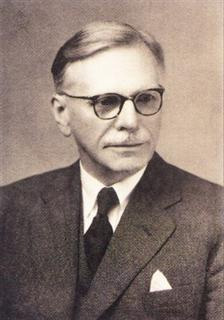
\includegraphics[width=.9\textwidth]{figures/John_Rupert_Firth.jpg}
  \caption{John Rupert Firth}
  \label{fig:ch.firth.firth_wiki}
\end{wrapfigure}
This notion that some phonological properties are not uniquely
`placed' with respect to particular segments within a larger unit is
the beginning of the notion of \emph{\isi{prosody}} which plays such a central role
in Firthian phonology. It represents the first substantial challenge
within twentieth-century linguistics to the notion that division of
the utterance into phonetic segments provides the essential basis for
further analysis, and that the analysis can then proceed exclusively
as a matter of assigning particular properties of the phonetic
material to particular segments.

Indeed, {\Firth} obviously had grave reservations about the validity of
\isi{segmentation} in general. In two postwar papers dealing with the
techniques of phonetic analysis
\citep{firth48:palatograms,firth50:palatography}, he discusses the
phenomenon of \isi{coarticulation} (the mutual interleaving of the phonetic
properties associated with distinct segments, so that no moment in
time can be regarded as uniquely representing the properties of a
single segment) and suggests that a segmental analysis both ignores
the fine detail of \isi{articulation} and paints a false picture by
suggesting that speech is divided into discrete temporal units.

He seems also to have been impressed by the possibility of certain
phonetic techniques which appear to reveal properties of stretches of
speech that are necessarily longer than a single
segment. Palatography, for example, necessarily presents a unitary
picture for an entire utterance (minimally, a single \isi{syllable}): if the
properties revealed in palatograms are relevant and interesting, he
appears to be saying, they suggest something other than segmental
analysis because of their intrinsically `unplaced' character. A number
of papers by {\Firth}'s students also appeal to palatographic evidence
(as well as kymography, to the virtual exclusion of other instrumental
phonetic techniques).

The central paper in the development of \isi{prosodic analysis} is generally
taken to be ``Sounds and Prosodies'' \citep{firth48:sounds:prosodies},
though it would perhaps be difficult for the modern reader to see how
this could be regarded as establishing a coherent program of research
without the benefit of subsequent exegesis such as that provided by
\citet{robins:prosodic,robins:ling_in_gb},
\citet{lyons62:non-phonemic}, and \citet{palmer70:prosodic}. The paper
starts from the observation that we can recognize different domains
within an utterance in which phonetic properties are distributed. Some
occur over fairly long stretches: intonation, for example,
characterizes an entire sentence (or at least an intonational phrase);
\isi{stress} patterns typically characterize an entire word; and tonal
elements are generally distributed over an entire \isi{syllable}. These
properties are all of the sort often bracketed by phonologists as
`suprasegmental', but {\Firth} suggests that if we take the possibility
seriously, we will find the same phenomenon in more classically
segmental domains, such as the properties of \isi{yotization} and
\isi{labiovelarization} he had earlier proposed in his analysis of Hunan
\ili{Chinese}.

Recognizing this relation between properties and the structural
domains with\-in which they occur, we can distinguish two sorts of
relations in linguistic structure (a division parallel to those made
by {\Saussure}, {\Hjelmslev}, and others). On the one hand, some properties
serve to organize or delimit stretches within an utterance. These
\emph{syntagmatic} relations between different sub-parts of the same
utterance are what characterize (in {\Firth}'s usage) linguistic
\emph{structures} such as the organization of segments into syllables,
syllables into higher units such as words, intonational phrases,
etc. On the other hand, some properties serve as alternative
(non-co-occurring) possibilities at some point in a structure, and
function \emph{paradigmatically} to \isi{contrast} one linguistic form with
another. An inventory of the paradigmatic possibilities available at a
given position in a structure is the \emph{system} operative at that
position. The difference between structures and the systems which
function within them is a central \isi{concept} of Firthian phonology.

In providing an analysis of the phonological structure of a language,
several different aspects can be distinguished. Essentially, we can
identify three components of a phonologically analyzed form. First,
its basic syllabic structure can be specified in terms of an abstract
pattern of C and V (consonant and vowel) elements, without regard to
the particular phonetic identities of these. In his description of
Cairo colloquial \ili{Arabic} \citep{firth48:sounds:prosodies}, he notes
that such a characterization must specify the number of syllables;
their nature as open or closed; their quantity; and their sequential
order. All of this information can be represented as a sequential
arrangement of C's and V's.

Secondly, we can identify features which characterize or delimit
particular aspects of this structure; a property with this function is
called a \emph{prosody}. A given property may be treated as a prosody
because its manifestation extends over a number of positions within
the structure, such as the properties of \isi{yotization} or
\isi{labiovelarization} discussed earlier. Even if a property is only
realized at a single position in a structure, however, it is treated
as a prosody if its occurrence is specifically characteristic of that
position. For instance, in a language which has both aspirated and
plain \isi{consonants} in \isi{syllable} initial position, but only plain
\isi{consonants} elsewhere, it may be appropriate to establish a prosody of
\isi{aspiration} which is realized as \isi{aspiration} specifically of the
syllable-initial consonant (and whose absence implies non-\isi{aspiration}),
rather than positing both aspirated and plain \isi{consonants} in the
syllable-initial system. Such properties whose location is bound to a
particular point in a structure serve to demarcate the structure, and
not simply to characterize a paradigmatic element within it.

Finally, after the structure has been specified abstractly and the
prosodies associated with it identified, the residual paradigmatic
properties identifiable in particular positions can be organized into
systems. The elements of these systems (each corresponding to a single
structural position, and thus roughly segment-sized in their scope)
constitute the \emph{phonematic} units of the given position in the
structure. These \isi{phonematic units} can be called the \emph{sounds}
which co-occur in a structure with the various prosodies
characteristic of that structure.

This, in outline, is the nature of a \isi{prosodic analysis}: an
apportioning of the phonic data of utterances among the elements of
structure, prosodies associated with particular units of structure
(phrase, word, \isi{syllable}, or parts of syllables), which may form
systems connected with those units, and the \isi{phonematic units} which
form systems at individual points of structure. To give any sort of
feeling for the `flavor' of a prosodic treatment of linguistic facts,
it would clearly be necessary to go far beyond this mere sketch and
present some substantive body of analyses, but this falls outside the
scope of the present book. There are a few points we should make
about the nature of this theory before proceeding to compare it with
other phonological views, however.

We have presented the nature of a \isi{prosodic analysis} above as a sort of
\isi{deduction} based on the phonetic material (and the \isi{regularities} to be
found in it) alone; but it should be stressed that {\Firth} and his
students did not at all maintain a separation of phonological from
grammatical analysis. In fact, actual prosodic descriptions show
extensive grammatical conditioning. This follows in part from the
polysystemic nature of the analysis: the treatment of the phonology of
verbs, for example, may be completely separate from that of nouns, and
thus the statements in each part of the description are implicitly
conditioned by the category under discussion.

The notion of `\isi{major function}', too, introduces the possibility that
phonological differences may be directly linked (as in the case of
Ablaut or Umlaut phenomena) to grammatical differences. Statements of
particular elements in an analysis, too, could make use of as much
grammatical information as necessary: in
\posscitet{robins57:sundanese.nasality} description of nasality in
Sundanese, for example, a prosody of nasalization is specifically
defined to exclude a vowel which follows the plural infix marker from
its scope. This element is not phonologically distinguishable from
other sequences not involving the plural marker, and the phonological
statement thus must make direct reference to the identity of
particular morphological elements.

Since a \isi{prosodic analysis} was required merely to be `appropriate' to
the phonic data, and to `renew connection' with the language in the
sense of predicting data beyond the original corpus on which it was
based, there is no reason to expect that it would be recoverable from
the phonetic data alone. That is, the analyst could perfectly well
proceed in parallel on various aspects of the analysis, linking them
up where possible and making use of one part of the analysis in
another area where that seems useful. As a result, the grammatical and
phonological analyses will typically be interdependent: the test of an
adequate grammar is not whether (as for most American linguistics of
the same period—see chapter~\ref{ch.structuralists}) it is
unambiguously recoverable from the data alone, but whether the entire
grammar, once arrived at (perhaps by the application of rigorous
procedures, perhaps by divine inspiration), satisifes the
reiquirements that its terms have exponents in the phonic data and
that it renews connection with the language.

It would be perfectly possible, for example, for phonetically
identical material to have more than one phonological analysis: an
example cited by \citet{palmer70:prosodic} is the nonequivalence of
\emph{banned} and \emph{band} in \ili{English} despite their phonetic
identity. Such a rejection of the requirement that phonological and
\isi{phonetic representations} be mutually interconvertible in an
unambiguous fashion is a point shared by {\Firth} with {\Hjelmslev} (see
chapter~\ref{ch.hjelmslev} above), though {\Firth}'s opinion of {\Hjelmslev}
was that his writings were mere `linguistic philosophy'.

It is obvious that the syntagmatic dependencies described in Firthian
terms as prosodies are just the sort of regularity that generative
descriptions would capture in terms of rules. The prosody of
\isi{yotization}, for example, might be represented by a rule (or set of
rules) modifying the quality of vowels in syllables whose initial
consonant is basically palatalized. \citet{langendoen68:london.school}
surveys a number of prosodic analyses and provides interpretations of
their central features in terms of rules rather than prosodies. In his
criticisms of this reanalysis, \citet{robins69:rvw.langendoen} appears
to confuse two distinct issues: whether rules furnish a more
appropriate format for description than (static) prosodies, and
whether a description should be limited to the specification of only
the \isi{distinctive features} in a language. True, Langendoen\ia{Langendoen, D. Terrence}'s discussion
appears to reject those aspects of a prosodic account which bring out
the non-distinctive, sub-phonemic concomitants of distinctive
properties; but this is a fact about the particular (heavily
Jakobsonian) presuppositions of early generative work (see
chapter~\ref{ch.genphon} below) rather than a limitation inherent in
description of syntagmatic \isi{regularities} by means of rules.

By attempting to incorporate all of the syntagmatic \isi{regularities} of
language into an inventory of static representational elements (the
prosodies), Firthian analysis makes certain implicit claims about the
nature of these \isi{regularities} in natural languages. In particular,
since the relation between prosodies and their phonetic realizations
is the uniform one of exponence, it is impossible for one such prosody
to interact significantly with another in the ways represented in a
generative description by sequential application.

The essential content of the statement that `rule A precedes rule B'
is that information supplied by the operation of rule A is necessary
to the correct application of rule B (and on the other hand,
information which may be destroyed by the application of rule A is not
available to rule B). If all rules are represented by prosodies, and
these are defined as relations between a uniform level of structure
and its phonetic instantiations, there is no analog of the notion of
ordering. Therefore, any argument which tends to support the
linguistic significance of ordered application is \emph{a fortiori} an
argument against this particular conception of prosodies (though not,
of course, against the more general \isi{concept} of phonological elements
whose scope is not identifiable with a single segmental position).

In any event, it is quite clear that the Firthian \isi{prosodic analysis} is
entirely a theory of \isi{representations}; indeed several Firthian papers
cite as a virtue of their analysis the fact that it allows them to
avoid the rule-related notions of `\isi{assimilation}', `dissimilation', and
`action at a distance'. Regularities are incorporated into an analysis
exclusively in the form of definitions of representational elements
(structures, and the prosodic and phonematic elements that constitute
systems at various points within them). The \isi{representations} in
question are quite different from those countenanced by phonemic
theories, but they nonetheless have as their goal the interpretation
of phonological \isi{regularities} as elements of the representation of
particular forms rather than as rule-governed relations among forms.

\section{Relations between prosodic and other approaches to phonology}

In order to gain any sort of sense of how different in character Firthian prosodic
analyses are from most other approaches to \isi{sound structure}, the
interested reader can only be urged to consult papers such as those in
\citet{studies.in.linguistic.analysis} and
\posscitet{palmer70:prosodic} \textsl{Prosodic Analysis}. For the
historical purposes of the present book, however, it is important to
discuss the similarities and differences between \isi{prosodic analysis} and
some other theories. We make some comparisons below of the Firthian
approach with (a) classical structuralist \isi{phonemic theory}; (b)
{\Harris}'s theory of \emph{long components} within a phonemic analysis;
and (c) the theories of Autosegmental, Metrical, and Skeletal
phonology.

Comparisons between phonemic and \isi{prosodic analysis} are fairly easy to
make, since {\Firth} (and his students) quite explicitly saw the prosodic
theory as a more nearly adequate alternative to phonemics. {\Firth} at
least gave lip service to the idea that \isi{phonemic theory} had a role to
play in the design of orthographies and \isi{transcription} systems: anyone
who has read a prosodic description will have no trouble seeing that
however valid it may be scientifically, such a theory is unlikely to
serve as the basis of a practical writing system. Given his nominalist
philosophy of science (and the principle of polysystemic analysis),
there is no particular reason to doubt his sincerity in this regard,
though he certainly rejected the idea that phonemic analysis had any
scientific interest apart from such practical concerns.

Aside from the obvious difference in the nature of the \isi{representations}
posited, there are a number of other points distinguishing prosodic
from phonemic analyses. While one might be tempted to compare the
\isi{phonematic units} of the former with the phonemes of the latter, for
example, this would be a clear mistake. Both are essentially
segment-sized units, it is true, and form systems of paradigmatic
contrasts, but the similarities end there. In a phonemic analysis, all
of the distinctive properties of an utterance are apportioned among
the phonemes; while the \isi{phonematic units} of a \isi{prosodic analysis}
neither exhaust nor are limited to the distinctive or phonologically
relevant properties of a form. Prosodies too may represent distinctive
properties: if aspirated \isi{stops} are only possible in syllable-initial
position, for example, this may motivate the positing of a
syllable-prosody of \isi{aspiration}, in which case the distinction between
initial aspirated and plain \isi{stops} is a matter of prosodic \isi{contrast}
rather than a difference in \isi{phonematic units}.

Another important difference between prosodic and phonemic analyses
was alluded to above: the status of non-distinctive properties. Most
schools of phonemic analysis (and at least early generative phonology
as well) took the position that any property which does not serve to
distinguish forms from one another should be excluded from the
phonological description. At best, such properties are included in the
definitions of the allophonic realizations of phonological units, but
they certainly do not play a part in the definition of the primes of
phonological structure. Prosodic analysis, in {contrast}, is concerned
just as much with the non-distinctive as with the distinctive
properties. Prosodies are defined in terms of all of the systematic
syntagmatic \isi{regularities} that are associated with one another in a
given structure. In \posscitet{sprigg55:tibetan} analysis of \isi{tone} in
\ili{Tibetan}, for example, the exponents of either of the two tonal
prosodies include (a) features of vowel \isi{pitch}; (b) features of
duration of the vowel; (c) features of \isi{aspiration}, etc. in the initial
consonant; and (d) features of voice quality in the vowel. Only one of
these properties would need to be taken as distinctive, but all are
included in the definition of the prosodies.

The polysystemic nature of the analysis, involving as it does a
relativization of the system of contrasts established to particular
sub-parts of the language, furnishes another difference between
prosodic and phonemic approaches. In general, the goal of a phonemic
analysis is to establish a uniform system of phonemes for a given
language. The possibility that distinct alternative phonemic analyses
might be equally available for a given language was admitted
\citep{chao34:non-uniqueness}, but each such analysis was presumed to
be applicable to the language as a whole. Some writers recognized
so-called `coexistent phonemic systems' for limited sub-parts of the
vocabulary (typically, the loanwords which would otherwise be
problematic for the \isi{regularities} characterizing the core or native
vocabulary of a language), and at least \citet{twaddell35:on.defining}
recognized the possibility of establishing different systems of
\isi{contrast} for different structural positions, but these were both
marginal and controversial positions, and no phonemicist would have
admitted different systems for nouns and verbs, or most of the other
uses of grammatical conditioning made by prosodic analysts.

The issue might be stated as follows: phonemic analysts intended to
generalize a single (phonetically based) system across as much of the
language as possible, while Firthian treatments attempted to limit the
focus of each part of an analysis as narrowly as possible so as to
discover all of the existing syntagmatic \isi{regularities} of sound
structure—some of which may be restricted to very specific sub-parts of
the language, perhaps to grammatically determined contexts. There was
no need felt for all of these sub-parts of the analysis to be relatable
to a single overall system.

A development in phonemic analysis which has obvious similarities with
pro\-sodic treatments was
\posscitet{harris44:long.components,harris:methods} proposal to extend
such an analysis by the extraction of certain \emph{long
  components}. Essentially, this is a method for dealing with
limitations on the distribution of certain units in the phonemic
inventory. One may discover, for example, that in some language
clusters of obstruents must always have the same value for \isi{voicing}
throughout, although \isi{voicing} is generally independently contrastive:
thus, /st/ and /zd/ are possible, but not /sd/ or /zt/. In such a
case, one can say that \isi{voicing} is a property which extends over an
entire cluster, rather than being limited to a single segment. On this
basis, a \isi{long component} of \isi{voicing} can be extracted and treated as an
element of the phonemic system. The obstruents will now include only a
single dental fricative /S/ and a single dental stop /T/, with [z] and
[d] being treated as /S/ and /T/ combined with the \isi{long component}
\isi{phoneme} of \isi{voicing}.

Such an analysis bears an obvious similarity to the extraction of
prosodies, but there are differences as well. One of these follows
from the concentration of phonemic analysis on distinctive properties:
only contrastive features are extracted as long components in {\Harris}'s
analysis, while non-\isi{distinctive features} are just as eligible for
prosodic treatment as distinctive ones, if they display syntagmatic
\isi{regularities} of distribution. Further, if a property is extracted as a
\isi{long component} in one position (say \isi{voicing}, in the example just
mentioned), it is to be so treated in all positions: thus, all voiced
obstruents in such a language are treated as combinations of a
nonspecific obstruent with the component of \isi{voicing}. A prosodic
analysis, in \isi{contrast}, may extract a given feature as prosodic in one
position, but treat it as part of the definition of \isi{phonematic units}
in others. A final \isi{nasal consonant} may be treated as part of a
syllable-prosody of nasalization, for example, but serve as a
phonematic unit in initial position, as suggested already in
\posscitet{firth.rogers37:hunanese} analysis of Hunan \ili{Chinese}.

In \posscitet{robins69:rvw.langendoen} review of
\citet{langendoen68:london.school}, he argues that another
difference between \isi{long component} analysis and prosodies is that ``no
particular structures are identified with the domains of long
components, whereas it is cardinal for the abstraction of a prosody
that the feature or features assigned to it as its \isi{exponent}(s) should
either characterize or demarcate a definite structure.'' Perhaps this
is true in principle, but in practice Robins\ia{Robins, R. H.}'s claim is rather
dubious.

If we examine \posscitet{allen51:sanskrit} treatment of \isi{retroflexion}
in \ili{Sanskrit}, for example, it is indeed possible to say that the
R-prosody he identifies is a property of the word; but its actual
domain is only a particular consonant or cluster, or a stretch
extending from an instance of \emph{r} (syllabic or not) or \emph{ș}
(retroflex \emph{s}) through as many following segments as possible
until a dental or palatal consonant other than \emph{n} is
encountered. The actual domain demarcated by this prosody is in no
interesting sense coextensive with an independently motivated
structural unit. Similarly, \isi{vowel harmony} in \ili{Turkish} may (in the
general case) extend from any arbitrary structural position to any
other within the word. This prosody does not respect morpheme
\isi{boundaries} (the element -\emph{Iyor}- `progressive', for example, has an
initial vowel that harmonizes with preceding vowels, but a second
vowel which initiates a new span of back, rounded harmony); neither
does it necessarily characterize an entire word, or have a scope whose
\isi{boundaries} necessarily coincide with the \isi{boundaries} of a word.

Both in spirit and in execution, \isi{prosodic analysis} is very different
from phonemic analysis (with or without the addition of long
components). It is, however, somewhat closer to some recent generative
work. The emphasis on enriched notions of phonological representation
which produced the theories of Autosegmental, and Metrical phonology
(chapter~\ref{ch.otlabphon}) resulted in analyses which are strikingly
like prosodic treatments. It is interesting to read
\posscitet{palmer70:prosodic} comment on {\Firth}'s analysis of \ili{Arabic}
structure, which extracted as separate formal aspects (a) a set of
properties of \isi{syllable} structure, summarized as a sequence of C's and
V's; (b) the sequence of \isi{consonants}; (c) the sequence of vowels; (d)
the position, nature, and quantity of the prominent; and (e) the clear
or dark qualities of the syllables. Palmer\ia{Palmer, Frank R.} calls this ``quite a
striking passage which may perhaps today no longer seem plausible,''
but the analysis proposed is virtually identical with that which an
influential paper by \citet{mccarthy81:prosodictheory} argues for
Classical \ili{Arabic}, with the exception of point \emph{e}, which McCarthy\ia{McCarthy, John J.}
does not discuss.

Similarly, a classic domain in which prosodic treatment is argued to
be particularly appropriate is the description of vowel (and
consonant) harmony systems, and here too the same systems have figured
in arguments for extracting some features from the segmental core as
autosegments \citep{goldsmith79:autosegmental}. Indeed, the same
properties of \isi{vowel harmony} systems have been used as arguments in
both cases. Thus \citet{sprigg61:vowel.harmony} argues that vowel
harmony in \ili{Tibetan} is better treated as prosodic than by rules of
segmental \isi{assimilation}, in part because the direction of the
\isi{assimilation} would be from right to left in some instances but from
left to right in others. This is exactly parallel to an argument made
by \citet{clements76:vowel.harmony} that \isi{vowel harmony} should be
described in autosegmental terms because (in the general case) it is
an essentially nondirectional process.

Autosegments in \isi{representations} are similar to prosodies,\footnote{The
  relations between Autosegmental and Prosodic Phonology are pursued
  by \citet{goldsmith92:prosodic}. The putative connections alleged by
  {\Goldsmith} and others are, however, rejected by
  \citet{ogden.local94:misrepresentation}, whose points are in some
  respects similar to ones made here.}  and metrical and skeletal
\isi{representations} are quite close to Firthian `structures' within which
systems of \isi{phonematic units} and prosodies operate.The notion of an
autosegment's being linked lexically to a particular segment, for
example, correspond closely to the Firthian notion that a prosody may
have a `focus'. There are some interesting differences as well,
however. For example, a prosody may extend over several structural
positions, just as an autosegment can, but there is no case in which
more than one prosody from the same system can be associated with the
same structural position, as in the autosegmental analysis of contour
\isi{tone}s (which involve two or more independent tonal autosegments
attached to the same vowel).

On the other hand, prosodic theory also allows a richer array of
possibilities in some respects than \isi{autosegmental theory}. A prosody,
for example, may involve any arbitrary combination of phonetic
properties, so long as they are systematically related to one another
in a syntagmatic way: thus \isi{aspiration}, \isi{tone}, \isi{length}, and \isi{voice quality}
(realized in different positions within the \isi{syllable}) are all part of
the same tonal prosodies in Sprigg\ia{Sprigg, Richard Keith}'s analysis of \ili{Tibetan}. An
autosegment, on the other hand, is simply a particular feature whose
relation to structural positions in the skeletal structure is not
necessarily one-to-one. It must thus be an individual, phonetically
coherent feature (though several separate autosegments may be
coordinated in their association with the segmental structure).

Another difference is that prosodies represent general syntagmatic
dependencies, whatever their nature, while \isi{autosegments} represent a
particular property with scope greater (or less) than a single
segment. \citet{allen51:sanskrit} describes the phenomena associated
with Grassman's law in \ili{Sanskrit} by means of a \isi{prosody} of \isi{aspiration},
for example, which represents a \emph{dis}-similatory relationship,
and thus could not be encoded in a similar way within an autosegmental
representation.

Aside from these points of detail, another major difference exists
between the two theories. \isi{Prosodic analysis}, as we noted above, is an
attempt to encode the effects of rules exhaustively within a theory of
static \isi{representations}. Autosegmental and metrical formalisms, on the
other hand, are simply theories of the \isi{representations} that appear
within a theory which contains significant rules as well. These rules
may manipulate autosegmental and metrical structure in various ways,
extending or contracting the scope of autosegmental associations,
changing one metrical structure into another (as in processes of
re-syllabification, for example), etc. One consequence of this
difference is that the extent of possible interrelation among
`prosodic' processes is much richer in this theory than in prosodic
analysis, which has no analog of even simple cases of rule
ordering. Other consequences of an enriched theory, in which
\isi{representations} not only are not limited to segmental ones but are
subject to rule-governed manipulation, have also been explored. A full
understanding of these formalisms, however, would undoubtedly benefit
from a study of the descriptive possibilities admitted by the rather
more limited, exclusively representational theory of Firthian prosodic
analysis.

%%% Local Variables: 
%%% mode: latex
%%% TeX-master: "/Users/sra/Dropbox/Docs/Books/P20C_2/LSP/main.tex"
%%% End: 
